% ----------------------------------------------------------------------------
% Vorlage Abschlussarbeit Informatik THM (minimal)
%
% Copyright (c) 2016 - 2020 by Burkhardt Renz. All rights reserved.
% Die Vorlage für eine Abschlussarbeit in der Informatik am Fachbereich
% MNI der THM ist lizenziert unter einer Creative Commons
% Namensnennung-Nicht kommerziell 4.0 International Lizenz.
%
% $Id: hausarbeit_vue.tex 979 2020-08-24 07:03:19Z br $
% ----------------------------------------------------------------------------

\documentclass[%
	BCOR=8.25mm,         % Bindekorrektur
	DIV=12,              % Satzspiegel
	parskip=half,				 % Abstand zwischen Absätzen
	bibliography=totoc,	 % Literaturverzeichnis im Inhaltsverzeichnis
	headsepline=on,      % Trennlinie Kolumnentitel
	]{scrbook}

%% Präambel
\usepackage[english, ngerman]{babel} % deutsche typogr. Regeln + Trenntabelle
\usepackage[T1]{fontenc}             % interner TeX-Font-Codierung
\usepackage{lmodern}                 % Font Latin Modern
\usepackage[utf8]{inputenc}          % Font-Codierung der Eingabedatei
\usepackage[babel]{csquotes}         % Anführungszeichen
\usepackage{graphicx}% Graphiken
\usepackage{float}
\usepackage{booktabs}                % Tabellen schöner
\usepackage{listingsutf8}            % Listings mit Einstellungen
\lstset{basicstyle=\small\ttfamily,
	tabsize=2,
	basewidth={0.5em,0.45em},
	extendedchars=true}
\lstset{literate=%                   % Umlaute in Listings
  {Ö}{{\"O}}1
  {Ä}{{\"A}}1
  {Ü}{{\"U}}1
  {ß}{{\ss}}2
  {ü}{{\"u}}1
  {ä}{{\"a}}1
  {ö}{{\"o}}1
	{~}{{\textasciitilde}}1} 
\usepackage{amsmath}	               % Mathematik
\usepackage[pdftex]{hyperref}       
\hypersetup{
	bookmarksopen=true,
	bookmarksopenlevel=3,
	colorlinks,
	citecolor=blue,
	linkcolor=blue,
}
\usepackage{scrhack}
\usepackage{bugtracker}								 % unterdrückt Fehlermeldung von listings

%js highlighting
\definecolor{lightgray}{rgb}{.9,.9,.9}
\definecolor{darkgray}{rgb}{.4,.4,.4}
\definecolor{purple}{rgb}{0.65, 0.12, 0.82}

\lstdefinelanguage{JavaScript}{
	keywords={typeof, new, true, false, catch, function, return, null, catch, switch, var, if, in, while, do, else, case, break},
	keywordstyle=\color{blue}\bfseries,
	ndkeywords={class, export, boolean, throw, implements, import, this},
	ndkeywordstyle=\color{darkgray}\bfseries,
	identifierstyle=\color{black},
	sensitive=false,
	comment=[l]{//},
	morecomment=[s]{/*}{*/},
	commentstyle=\color{purple}\ttfamily,
	stringstyle=\color{red}\ttfamily,
	morestring=[b]',
	morestring=[b]"
}

\lstset{
	language=JavaScript,
	backgroundcolor=\color{lightgray},
	extendedchars=true,
	basicstyle=\footnotesize\ttfamily,
	showstringspaces=false,
	showspaces=false,
	numbers=left,
	numberstyle=\footnotesize,
	numbersep=9pt,
	tabsize=2,
	breaklines=true,
	showtabs=false,
	captionpos=b
}

%% Nummerierungstiefen
\setcounter{tocdepth}{3}             % 3 Stufen im Inhaltsverzeichnis
\setcounter{secnumdepth}{3} 		     % 3 Stufen in Abschnittnummerierung

% ----------------------------------------------------------------------------
\begin{document}

\frontmatter

%% Titelseite
\begin{titlepage}
	\begin{center}
	
\includegraphics[width=0.9\textwidth]{img/mni-logo}
	
	\vspace{5cm}	

	\Large\textbf{\sffamily Hauptseminar-Arbeit}

	\vspace{1cm}	

	\huge\textbf{\sffamily Vue.js}

	\normalsize
	\vspace{1cm}

	Prüfungsleitung des Moduls \\
	CS1025 Hauptseminar

	von \\[1cm]	

	\textbf{Maximilian Biebl} \\ \texttt{Matrikelnr.: 5323481}\\ [.5cm]
	am \today
	\end{center}
	\vfill
	\begin{tabular}{ll}
		Dozent: & Sebastian Süß
	\end{tabular}
\end{titlepage}
\cleardoubleemptypage

%% Erklärung
\pagestyle{empty}
\begin{quote}
	\vspace*{4cm}

	\begin{center}
		\textbf{\Large\sffamily Eidesstattliche Erklärung}
	\end{center}

	Hiermit versichere ich, die vorliegende Arbeit selbstständig und unter
	ausschließlicher Verwendung der angegebenen Literatur und Hilfsmittel
	erstellt zu haben.

	Die Arbeit wurde bisher in gleicher oder ähnlicher Form keiner anderen
	Prüfungsbehörde vorgelegt und auch nicht veröffentlicht.

	\vspace{2em}
	
\includegraphics[scale=0.5]{img/signature}

	Limburg, \today
\end{quote}
\cleardoubleemptypage

%% Zusammenfassung
\pagestyle{empty}
\begin{quote}
	\vspace*{4cm}

	\begin{center}
		\textbf{\Large\sffamily Zusammenfassung}
	\end{center}
	Heutzutage ist es Standard, dass man mit einer Webseite interagieren kann und sich die Inhalte der Webseite dynamisch anpassen.
	Eine Webanwendung mit einer komplexen Benutzeroberfläche ohne die Verwendung eines Frontend-Frameworks zu entwickeln, ist aufwendig und fehleranfällig.
	Zudem besteht ein erhöhtes Risiko von Inkonsistenzen in Bezug auf Inhalt und Qualität, was die spätere Wartung erschwert.
	Für eine Webanwendung wird in der Regel ein Frontend-Framework verwendet, die aktuell gängigsten dieser Frameworks sind React, Angular und Vue.js.
	Diese Frontend-Frameworks bilden das Bindeglied zwischen der Logik in JavaScript und der Darstellung in HTML und CSS.
	In dieser Ausarbeitung möchten wir uns genauer mit dem Framework Vue.js beschäftigen und einen Vergleich zu React und Angular ziehen.

	
\end{quote}
\cleardoubleemptypage

%% Verzeichnissse
\tableofcontents

\listoffigures
\listoftables
\lstlistoflistings

\mainmatter 
\pagestyle{headings}
% ----------------------------------------------------------------------------
% Copyright (c) 2016 - 2020 by Burkhardt Renz. All rights reserved.
% Die Vorlage für eine Abschlussarbeit in der Informatik am Fachbereich
% MNI der THM ist lizenziert unter einer Creative Commons
% Namensnennung-Nicht kommerziell 4.0 International Lizenz.
%
% Id:$
% ----------------------------------------------------------------------------

\chapter{Frontend Frameworks}

In diesem Kapitel möchte ich zunächst allgemein in die JavaScript-Frontend-Frameworks einführen.
Die Drei aktuell gängigsten Frontend-Frameworks React.js, Angular und Vue.js werden vorgestellt.
\\
\\
An eine moderne Webapplikation werden hohe Anforderungen an den Funktionsumfang durch den Benutzer gestellt.
Die Entwickler einer solchen Webapplikation erwarten eine einheitliche Codequalität und einheitliche Strukturen
für eine bessere Wartbarkeit der Webapplikation.
Um beim Erstellen neuer Webapplikationen den Entwickler dabei zu unterstützen diese Ziele zu erfüllen,
werden unter anderem entsprechende Frontend Frameworks verwendet.
\begin{quote}
    Front-end frameworks determine the logic, structure, design, behavior,
    and animation of every element you see on-screen when you interact with websites,
    web applications, and mobile apps. \cite{sigdestad22}
\end{quote}
Man kann zwischen UI-Frameworks in HTML und CSS sowie JavaScript-Frameworks unterscheiden.
Letztere dienen als Verbindung zwischen der Darstellung und der Logik im Frontend.
Aus den Statistiken \ref{fig:stackoverflow_stat} und \ref{fig:google_trends} lässt sich schließen,
dass die Drei aktuell gängigsten dieser JavaScript-Frameworks React.js, Angular und Vue.js sind.

%TODO DOM erklären


\begin{figure}[!htb]
    \centering
    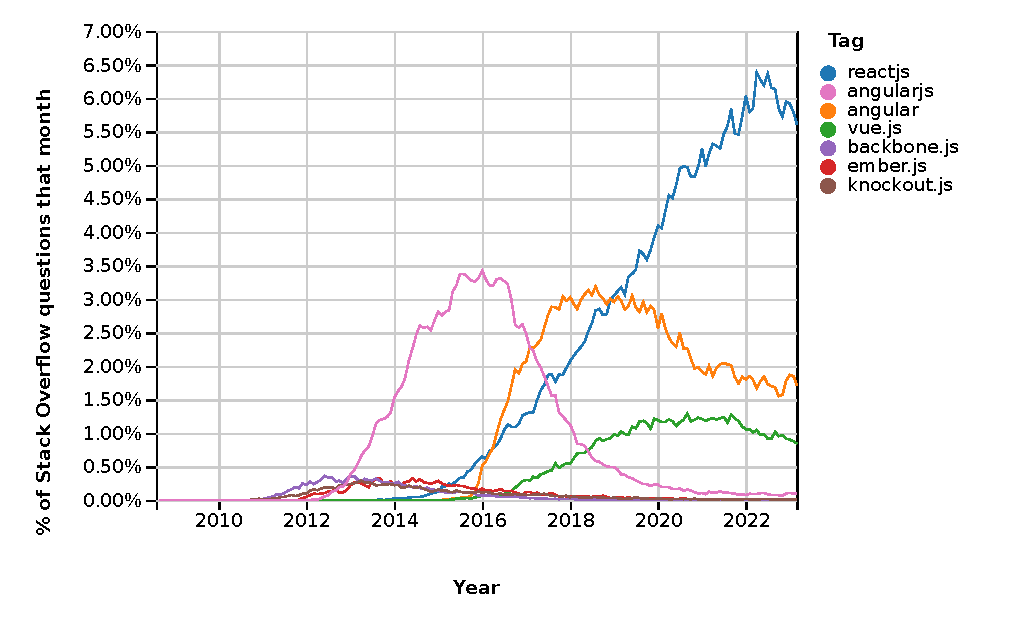
\includegraphics[width=0.8\textwidth]{img/js_frameworks_statistic_stackoverflow}
    \caption{Stackoverflow Statistik zur Häufigkeit von Fragen nach Framework \cite{stackoverflowStats}}
    \label{fig:stackoverflow_stat}
\end{figure}

\begin{figure}[!htb]
    \centering
    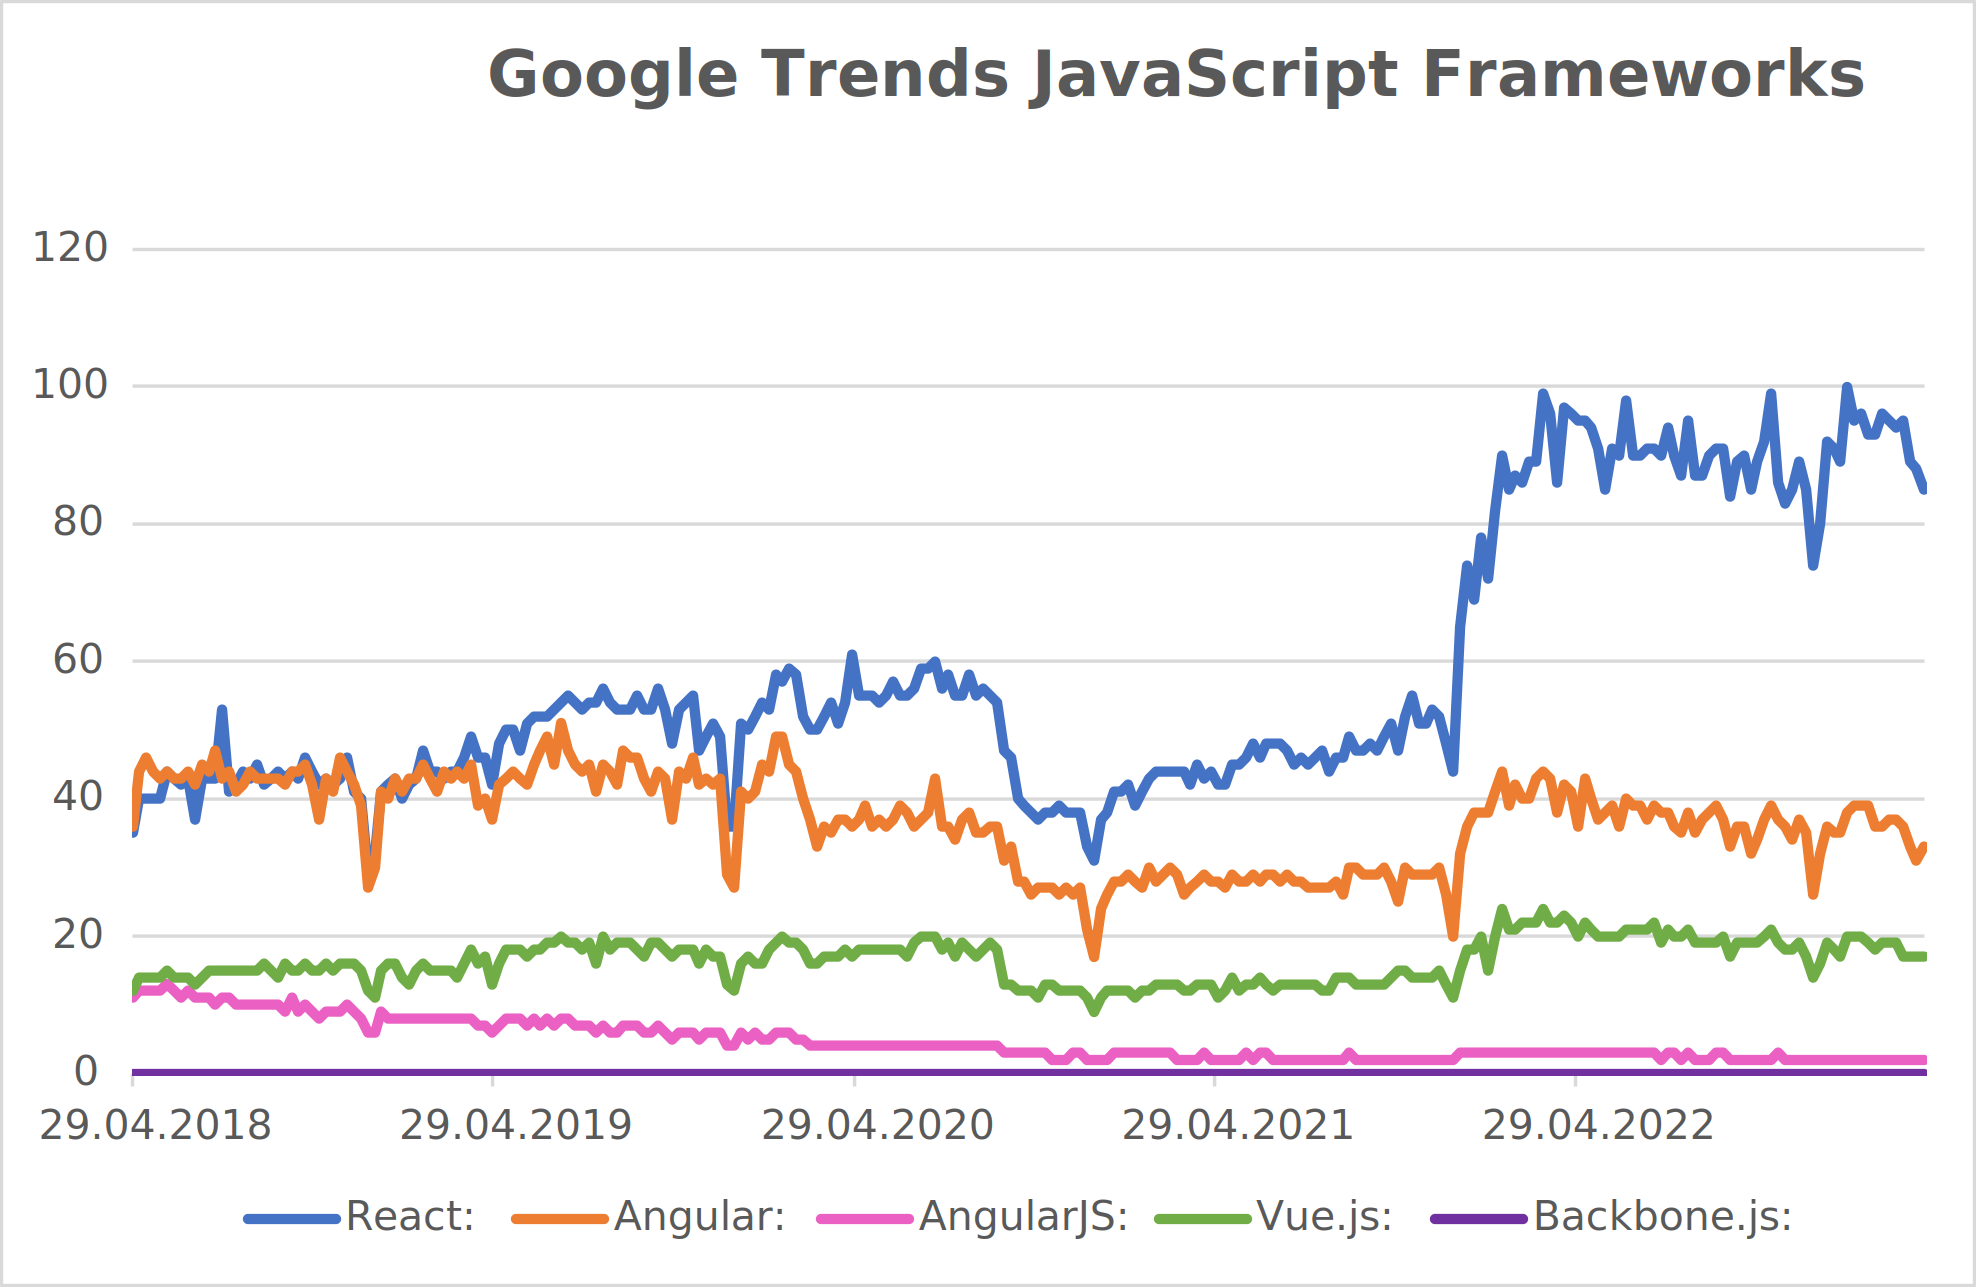
\includegraphics[width=0.8\textwidth]{img/Google Stats/google_frameworks_trends}
    \caption{Googlge Trends zur Häufigkeit von Suchanfragen nach Frameworks der letzten 5 Jahre \cite{googleTrends}}
    \label{fig:google_trends}
\end{figure}


\section{Vue.js}
Vue.js wurde von Evan You als Nebenprojekt entwickelt und erschien 2014.
Das Projekt finanziert sich laut eigenen Angaben aus Spenden und
wird von sowohl Vollzeitentwicklern und Freiwilligen gepflegt \cite{vueFAQ}.
Nach Google Trends und Stackoverflow Statistik ist es aktuell das drittbeliebteste
Frontend Framework \cite{googleTrends} \cite{stackoverflowStats}.
Hohe beliebtheit hat das Framework in China (siehe Abb.\ref{fig:google_trends_world}).
Besonderheit des Frameworks ist, dass es in seiner Grundform keine 20 KB groß ist \cite[S. 523]{bin2019}.


\section{Angular}
Angular wurde von Google entwickelt und erschien 2016 ursprünglich als \emph{AngularJs 2.0},
dabei handelt sich um eine vollständige Neuimplementierung in TypeScript unabhängig der Codebasis des Vorgängers AngularJs.
Die Pflege und Weiterentwicklung wird vom Angular Team von Google durchgeführt \cite[S. 209-210]{bin2019}.
Nach Google Trends und Stackoverflow Statistik ist es aktuell das zweitbeliebteste
Frontend Framework \cite{googleTrends} \cite{stackoverflowStats}.

\newpage

\section{React.js}
Das laut Stackoverflow Statistik und Google Trends gefragteste Frontend Framework ist aktuell React.js \cite{googleTrends} \cite{stackoverflowStats}.
React.js wurde von Facebook entwickelt und 2013 veröffentlicht.
Das Ziel bestand darin, ein Framework zu entwickeln,
das den Anforderungen an Skalierbarkeit und Wartbarkeit gerecht wird,
wie sie für eine umfangreiche Webapplikation wie Facebook erforderlich sind \cite[S. 1]{gackenheimer2015introduction}.
Mittlerweile ist es ein Open-Source-Projekt des Facebookmutterkonzerns Meta.
React setzt dabei auf \emph{JavaScript syntax extension} (JSX) was einen hybriden Code aus JavaScript und HTML-Elementen ermöglicht. \cite{react}


\begin{figure}[!htb]
    \centering
    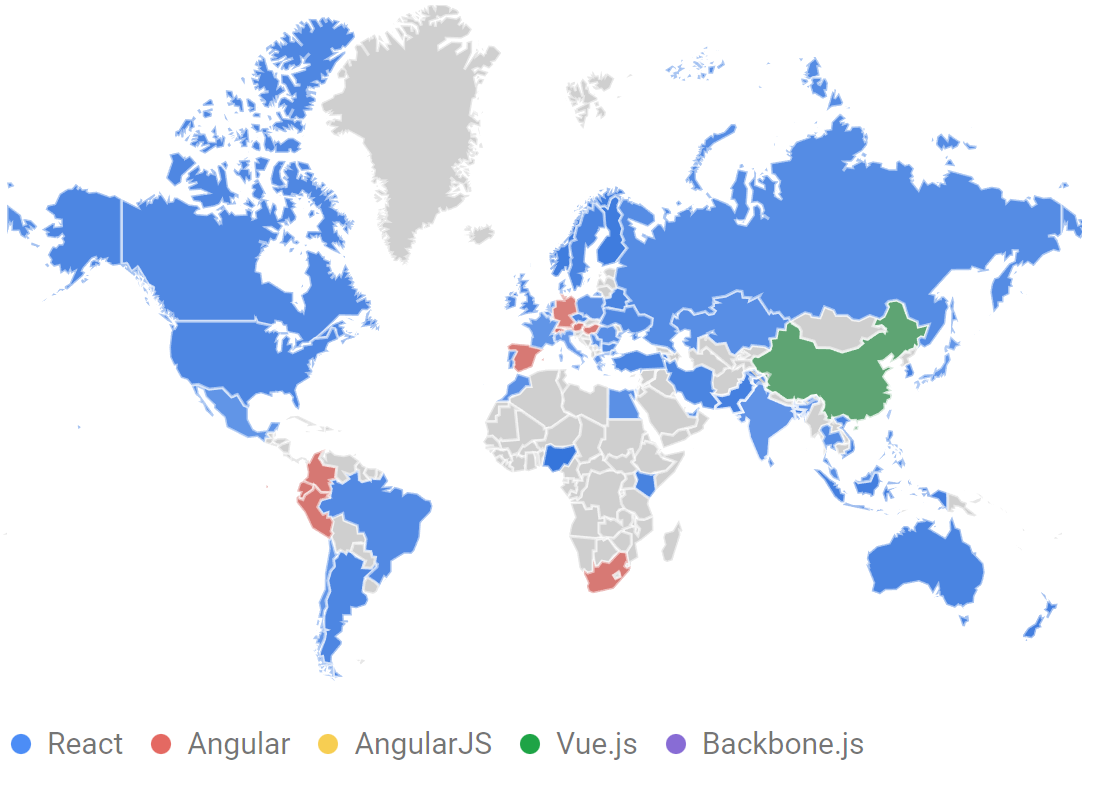
\includegraphics[width=0.6\textwidth]{img/Google Stats/2023-04-26 12_20_26-React, Angular, AngularJS, Vue.js, Backbone.js - Erkunden - Google Trends}
    \caption{Googlge Trends Weltweiteverteilung von Suchanfragen nach Frameworks der letzten 5 Jahre \cite{googleTrends}}
    \label{fig:google_trends_world}
\end{figure}
% ----------------------------------------------------------------------------

%! Author = biebl
%! Date = 28.04.2023

\chapter{Vue.js}
In diesem Kapitel möchte ich genauer auf Vue.js eingehen.
Dabei möchte ich ausführlich auf Vue.js und seine Ziele eingehen.
Weiterhin möchte ich auf die Historie und Meilensteine in der Entwicklung von Vue.js erläutern.


\section{Was ist Vue.js?}
Bei Vue handelt es sich um ein progressives JavaScript Frontend Framework.

\section{Geschichte}
%! Author = biebl
%! Date = 02.05.2023


\chapter{Technische Details}\label{ch:technische-details}
In diesem Kapitel soll es um die technischen Details von Vue.js gehen.
Es wird ein Überblick gezeigt von verschiedenen in Vue.js vorhandenen Elementen
und es wird auf diese anhand von Beispielen genauer eingegangen.
Die Betrachtung bezieht sich auf Vue 3.
Aufgrund der Kürze der Arbeit und des Funktionsumfangs von Vue.js ist es nicht mögliche alle Features abzudecken.
Das Kapitel dient dazu, dem Leser einen ersten Eindruck von Vue.js zu geben.


\section{Options API vs. Composition API}\label{sec:options-api-and-composition-api}
Vue.js organisiert einzelne Komponenten als \emph{Single-File Components (SFC)},
die im HTML-ähnlichen Dateiformat mit der Dateiendung \texttt{.vue} vorliegen.
In einem SFC werden Aussehen, Struktur und Logik einer Komponente gebündelt, bestehend aus HTML-, CSS- und JavaScript-Elementen.
Für den Aufbau einer solchen SFC gibt es seit Vue 3 zwei verschiedene Möglichkeiten.
Zum einen gibt es die \emph{Options API} und zum anderen die \emph{Composition API}. \cite{vueIntroduction}

\subsection*{Options API}
Die länger vorhandene Variante ist die Options API.
Bei der Options API wird für die Komponente ein JavaScript Objekt angelegt.
Das Objekt kann verschiedene Optionen enthalten, darunter \texttt{data} für Daten, \texttt{methods} für Methoden und auch Lifecycle-hooks wie \texttt{mounted}.
\cite{vueIntroduction}

\subsection*{Composition API}
Die Composition API kam mit Vue 3 hinzu und wurde später für Vue 2 nachgereicht \cite{vueFAQ}.
Bei der Verwendung der Composition API werden in einem \texttt{import}-Statement
die benötigten API-Features wie zum Beispiel Lifecycle-hooks angegeben.
Der Code bei Verwendung der Composition API wird in der Regel zwischen einem \texttt{<script setup>} Tag verwendet.
Durch die Verwendung des Tags wird zur Compilezeit eine Transformation durchgeführt,
die es ermöglicht, die Composition API mit weniger redundantem Code zu nutzen.
Somit ist es möglich, Variablen und Funktionen direkt im Template zu verwenden.
\cite{vueIntroduction}

\subsection*{Gegenüberstellung}

\begin{minipage}[t]{.45\textwidth}
    \begin{lstlisting}[caption={Options API},language=javascript, label={lst:OptionsAPI}]
<script>
export default {
  // reactive state
  data() {
    return {
     wasPressed : false
    }
  },

  // functions that mutate state and trigger updates
  methods: {
    setStatus() {
      this.wasPressed = true
    }
  },

  // lifecycle hooks
  mounted() {
    console.log(`mounted`)
  },

  update(){
    console.log(`update`)
  },

  unmounted(){
    console.log(`unmounted`)
  }
}
</script>

<template>
  <button @click="setStatus">Button was Pressed: {{ wasPressed }}</button>
</template>
    \end{lstlisting}
\end{minipage}%
\hspace{1cm}
\begin{minipage}[t]{.5\textwidth}
    \begin{lstlisting}[caption={Composition API},language=javascript, label={lst:CompositionAPI}]
<script setup>
import { ref, onMounted, onUpdated, onUnmounted } from 'vue'

// reactive state
const wasPressed = ref(false)

// functions that mutate state and trigger updates
function setStatus() {
  wasPressed.value = true;
}

// lifecycle hooks
onMounted(() => {
   console.log(`mounted`)
})

onUpdated(() => {
   console.log(`updated`)
})

 onUnmounted(() => {
   console.log(`unmounted`)
})

</script>

<template>
  <button @click="setStatus">Button was Pressed: {{ wasPressed }}</button>
</template>
    \end{lstlisting}
\end{minipage}

In Vue.js können beide APIs ohne Einschränkung genutzt werden.
Hier sind zwei gleichwertige Beispiele in \ref{lst:OptionsAPI} und \ref{lst:CompositionAPI} dargestellt,
die jeweils mit einer der APIs implementiert wurden.
Es werden Veränderungen im Lifecycle auf der Konsole ausgegeben und es wird festgehalten, ob ein Button gedrückt wurde.
Für Anfänger mit ersten Erfahrungen in Objektorientierung wird die Options API empfohlen.
Ansonsten sollte die Options API nur bei weniger komplexen Kleinprojekten genutzt werden.
Für größere Projekte wird die Composition API empfohlen. \cite{vueIntroduction}

\subsection*{Fazit zu Options API vs. Composition API}
Die Composition API ist deutlich übersichtlicher, strukturierter und spart redundanz im Code.
Auch bei weniger komplexen Kleinprojekten könnte sich die Options API als ungeeignet erweisen,
da unvorhergesehene Größenänderungen dazu führen können,
dass die wartbare Composition API die bessere Wahl ist.
Die Composition API ist der Options API vorzuziehen.


\section{Direktiven in Vue.js}\label{sec:direktiven-in-vue.js}
Direktiven beschreiben ein gewünschtes Verhalten in der View.
In Vue.js beginnen diese Direktiven mit \texttt{v-}.
Vue.js bietet einige vordefinierte Direktiven wie \texttt{v-for}, \texttt{v-if}, \texttt{v-else}, \texttt{v-show}, \texttt{v-on}, \texttt{v-slot}, \texttt{v-bind}
und \texttt{v-model}, bietet aber auch die Möglichkeit, eigene Direktiven zu erstellen. \cite[S. 10]{steyer2019}
\\
Es wird sich auf eine Auswahl der vordefinierten Direktiven beschränkt.
Eine Liste aller Direktiven\footnote{\url{https://vuejs.org/api/built-in-directives.html}}
und wie man eigene Direktiven\footnote{\url{https://vuejs.org/guide/reusability/custom-directives.html}}
erstellt, ist in der Dokumentation von Vue.js zu finden.
Auf Direktiven zur Datenbindung wird an passenderer Stelle in Abschnitt \ref{sec:datenbindung-in-vue.js} eingegangen.


\subsection*{v-for}
\texttt{v-for} funktioniert wie eine foreach-Schleife.
Die \texttt{v-for}-Direktive ermöglicht es über eine Sammlung von Werten zu iterieren und die Daten in der View zu nutzen.
Erlaubte Datentypen sind \texttt{Array}, \texttt{Object}, \texttt{number}, \texttt{string} und solche, die das Interface \texttt{Iterable} implementieren. \cite{vueDirectives}
\begin{lstlisting}[caption={\texttt{v-for}-Direktive},language=html, label={lst:v-for}]
<div v-for="element in list">
  {{ element.value }}
</div>
\end{lstlisting}

%\newpage

\subsection*{v-if}
Die Direktive \texttt{v-if} ähnelt in der Funktionsweise einem if-Statement in der Programmierung.
\texttt{v-if} prüft anhand des übergebenen Wahrheitswerts, ob ein HTML-Element angezeigt werden soll.
Mit der Verwendung von \texttt{v-if} können Alternativen mit \texttt{v-else} für den Fall, dass die Bedingung nicht erfüllt ist,
oder mit \texttt{v-else-if} für eine bedingte Alternative ergänzt werden.
Entsprechend dem Wahrheitswert werden dann die Alternativen angezeigt. \cite{vueDirectives}
\begin{lstlisting}[caption={\texttt{v-if}-Direktive},language=html, label={lst:v-if}]
<div v-if="condition">
  condition is true
</div>
<div v-else-if="anotherCondition">
  anotherCondition is true
</div>
<div v-else>
  condition and anotherCondition are false
</div>
\end{lstlisting}

\subsection*{v-on}
Mit der \texttt{v-on}-Direktive wird ein Event-Listener an das HTML-Element gebunden.
Die Direktive erhält als Argument das Event, auf das der Listener reagieren soll,
sowie die darauf auszuführende Aktion.
Als Kurzform von \texttt{v-on} ist auch \texttt{@} möglich.
Mit \texttt{\$event} ist es möglich Eventeigenschaften weiter zugeben.
Darüber hinaus gibt es noch Modifier, die das zu erwartende Event präzisieren. \cite{vueDirectives}
\begin{lstlisting}[caption={\texttt{v-on}-Direktive},language=html, label={lst:v-on}]
<button v-on:click="buttonClicked"></button>
<button @click="buttonClickedButShortHand"></button>
<button v-on:click.right="buttonRightClicked"></button>
\end{lstlisting}

%\newpage


\section{Komponenten in Vue.js}\label{sec:komponenten-in-vue.js}
Komponenten sind wiederverwendbare Bausteine.
Die Komponenten können beliebig oft in der View verwendet werden und im Model unabhängig angesteuert werden.
Vue.js bietet die Möglichkeit, Komponenten selbst aus HTML, CSS, sowie JavaScript zu definieren und sie später mit einem
selbst definierten HTML-Tag anzusteuern. \cite[S. 11-12]{steyer2019}
\\
Wie in Abschnitt \ref{sec:options-api-and-composition-api} bereits erwähnt, werden in Vue.js Komponenten normalerweise als SFC geschrieben.
Eine Komponente kann wie in Abschnitt \ref{sec:options-api-and-composition-api} erwähnt mit Composition API oder Options API
erstellt werden.
Alternativ kann man die Komponente als JavaScript Objekt erstellen, um den Build-Schritt zu umgehen (siehe Listing \ref{lst:Komponente als JavaScript-Objekt}).
Eine Komponente kann dann mit einem Alias im Script-Teile einer anderen Komponente importiert werden und muss dort noch als Komponente
registriert werden.
Nach dem Registrieren kann der Alias als Tag für die importierte Komponente verwendet werden. \cite{vueComponents}

\newpage

\begin{lstlisting}[caption={Komponente als JavaScript Objekt},language=javascript,label={lst:Komponente als JavaScript-Objekt}]
export default {
  data() {
    return {
     wasPressed : false
    }
  },
  template:`<button @click="setStatus">Button was Pressed: {{ wasPressed }}</button>`
}
\end{lstlisting}


\begin{lstlisting}[caption={Verwendung einer Komponente},language=javascript,label={lst:Verwendung einer Komponente}]
<script>

import ButtonStatusChecker from './ButtonStatusChecker.vue' //import of component

export default {
  components: {
    ButtonStatusChecker //component registration
  }
}
</script>

<template>
  <ButtonStatusChecker /> //using component
</template>
\end{lstlisting}

Neben der lokalen Registrierung existiert die Möglichkeit eine Komponente global
zu registrieren, um sie nicht bei jeder Verwendung in einer anderen Komponente
extra importieren und registrieren zu müssen.
Die globale Registrierung ist mit Aufruf der \texttt{component()}-Methode der App-Instanz möglich.
Der \texttt{component()}-Methode wird dann der Alias und die importierte \texttt{.vue}-Datei übergeben.
Alternativ kann auch die Implementierung beim Aufruf direkt übergeben werden. \cite{vueComponentsRegistration}

%\newpage

\begin{lstlisting}[caption={Globale Registrierung einer Komponente},language=javascript,label={lst:Globale Registrierung}]
import { createApp } from 'vue'
import ButtonStatusChecker from './ButtonStatusChecker.vue'
const app = createApp({})
app.component('ButtonStatusChecker', ButtonStatusChecker)
\end{lstlisting}


Um Daten an eine Komponente zu übergeben, gibt es die \texttt{props}-Option beim Erstellen einer Komponente.
Das \texttt{props}-Attribut erhält einen Namen, über die es dann später in
HTML angesteuert werden kann. \cite{vueComponents}

\newpage

\begin{lstlisting}[caption={Erstellung eines \texttt{props}},language=javascript,label={lst:Erstellung eines props}]
<script>
export default {
  props: ['text']
}
</script>

<template>
  <p>{{ text }}<p>
</template>
\end{lstlisting}

\begin{lstlisting}[caption={Nutzung eines \texttt{props}},language=javascript,label={lst:Nutzung eines props}]
<Paragraph text="Hallo Welt" />
\end{lstlisting}

Abgesehen von den bereits aufgezählten Features, bietet Vue.js für Komponenten weitere Features wie die Möglichkeit auf Events zu reagieren,
die Verwendung dynamischer Komponenten und Inhalte mittels \texttt{<slot>} an eine Komponente zu übergeben.
Eine Anleitung zur Verwendung dieser Features ist in der Vue.js Dokumentation nachzulesen\footnote{\url{https://vuejs.org/guide/essentials/component-basics.html}}.
\cite{vueComponents}

%\newpage


\section{Datenbindung in Vue.js}\label{sec:datenbindung-in-vue.js}
Das Binding ist einer der Hauptaufgaben eines Frontend Frameworks.
Beim Binding geht es darum, Daten von View und Model aneinander zubinden. \cite[S. 11]{steyer2019}
\subsection*{Mustache-Syntax}
Die einfachste Form der Datenbindung in Vue.js ist mit der auch aus anderen Frameworks bekannten Mustache-Syntax möglich.
Bei der Mustache-Syntax wird ein Variablenname aus dem Modell in der Komponente zwischen vier geschweifte Klammern gesetzt (siehe Listing \ref{lst:Mustache-Syntax}).
Angezeigt wird dann die aktuelle String-Repräsentation des Wertes.
Die Mustache-Syntax ist unidirektional vom Model zur View. \cite{vueTemplateSyntax}
\begin{lstlisting}[caption={Mustache-Syntax},language=javascript, label={lst:Mustache-Syntax}]
<script>
export default {
  data() {
    return {
     text : 'Hallo Welt'
    }
  }
</script>

<template>
  <p>{{ text }}</p>
</template>
\end{lstlisting}

\subsection*{v-text}
Neben den in Abschnitt \ref{sec:direktiven-in-vue.js}
erwähnten Direktiven gibt es noch weitere Direktiven zur Datenbindung.
Die \texttt{v-text}-Direktive ist eine Alternative zur Mustache-Syntax,
diese überschreibt jedoch den gesamten existierenden Inhalt des HTML-Elements bei einer Änderung im Model.
Eine Änderung in Teilen wie bei der Mustache-Syntax ist nicht möglich. \cite{vueDirectives}
\begin{lstlisting}[caption={\texttt{v-text}-Direktive},language=javascript, label={lst:v-text-Direktive}]
<script>
export default {
  data() {
    return {
     text : 'Hallo Welt'
    }
  }
</script>

<template>
  <p v-text="text"></p>
</template>
\end{lstlisting}

\subsection*{v-html}
Die \texttt{v-html}-Direktive erlaubt es, Daten aus dem Model in der View als HTML interpretieren zu lassen.
Aus Sicherheitsgründen empfiehlt es sich nur HTML-Code aus vertrauenswürdigen Quellen zu nutzen. \cite{vueTemplateSyntax}
\begin{lstlisting}[caption={\texttt{v-html}-Direktive},language=javascript, label={lst:v-html-Direktive}]
<script>
export default {
  data() {
    return {
     heading : '<h1>Hallo Welt</h1>'
    }
  }
</script>

<template>
  <p v-html="heading"></p>
</template>
\end{lstlisting}

\subsection*{v-bind}
Um Daten an HTML-Attribute zubinden, gibt es die \texttt{v-bind}-Direktive.
Da \texttt{v-bind} eine häufig genutzte Direktive ist, gibt es eine Kurzform,
die aus einem vorangestellten Doppelpunkt besteht. \cite{vueTemplateSyntax}
\begin{lstlisting}[caption={\texttt{v-bind}-Direktive},language=javascript, label={lst:v-bind-Direktive}]
<script>
export default {
  data() {
    return {
     id : 'greeting',
     idShortHand : 'target',
     isButtonOn: false
    }
  }
</script>

<template>
  <p v-bind:id="id">Hallo</p>
  <p :id="idShortHand">Welt</p>
  <button :disabled="isButtonOn">Drück mich</button>
</template>
\end{lstlisting}

%\newpage

\subsection*{v-model}
Die bisher vorgestellten Binding Varianten sind unidirektional,
für bidirektionales Binding gibt es die \texttt{v-model}-Direktive.
Die \texttt{v-model}-Direktive ist eine Verbindung aus \texttt{v-on}-Direktive
und \texttt{v-bind}-Direktive.
Mit der \texttt{v-bind}-Direktive ist es zum Beispiel möglich, vorausgefüllte Inputfelder zu erstellen.
Bei Eingabe in das Inputfeld wird entsprechend das Datenfeld im Modell aktualisiert
und bei Änderungen im Modell wird der Text im Inputfeld aktualisiert. \cite{vueComponentV-model}
\begin{lstlisting}[caption={\texttt{v-model}-Direktive},language=javascript, label={lst:v-model-Direktive}]
<script>
export default {
  data() {
    return {
     username : 'Mustermann',
    }
  }
</script>

<template>
  <input v-model="username" />
</template>
\end{lstlisting}

\newpage


\section{Routing in Vue.js}\label{sec:routing-in-vue.js}
Für das Routing muss man zwischen Multi-Page und Single-Page Anwendungen unterscheiden.
Bei einer Multi-Page Anwendung (MPA) erfolgt das Aufrufen einer neuen Unterseite über die Kommunikation
mit dem Server, die Seite wird dann serverseitig gerendert.
Bei MPA handelt es sich um einen älteren Ansatz.\cite[S. 262]{kaluvza2018comparison}
\\
In Vue.js wird der Ansatz der Single-Page Anwendung (SPA) verfolgt.
Bei Single-Page Anwendungen existieren Unterseiten nur simuliert und
die Inhalte einer einzelnen Seite werden mithilfe von JavaScript ausgetauscht. \cite[S. 174-175]{peterke2019}
\subsection*{Installation}
Der offizielle Router von Vue.js ist nicht Teil des Vue-Kerns und
muss daher bei Bedarf gesondert installiert werden.
Die aktuelle mit Vue 3 kompatible Router-Version ist Version 4 und
kann über npm mit dem Befehl \texttt{npm install vue-router@4} installiert werden.\cite{vueRouterInstallation}

%\newpage

\subsection*{Router initialisieren}
Man muss den Router zunächst erstellen.
Dem Router werden die Routen, bestehend aus Pfad und aufzurufender Komponente übergeben.
Zusätzlich wird beim Erstellen des Routers angegeben, wie die Routinghistorie festgehalten werden soll.
Abschließend muss der Vue-App-Instanz mitgeteilt werden, dass sie den Router nutzen soll. \cite{vueRouterGettingStarted}
\begin{lstlisting}[caption={Router initialisieren},language=javascript, label={lst:Router-initialisieren}]
//import of components
import Home from './Home.vue'
import About from './About.vue'

//define the routes
const routes = [
  { path: '/', component: Home },
  { path: '/about', component: About },
]

//create the router instance
const router = VueRouter.createRouter({
  history: VueRouter.createWebHashHistory(), //history mode
  routes: routes,
})

// creat app instance
const app = Vue.createApp({})
app.use(router)
app.mount('#app')
\end{lstlisting}

\subsection*{Verwendung des Routers}
Um den Router zu verwenden und auf eine neue Unterseite zu verlinken,
gibt es den HTML-Tag \texttt{router-link}, mit dem Attribut \texttt{to} kann dann der gewünschte Pfad angegeben werden.
Wie bereits erwähnt, verwendet man Vue.js in der Regel für SPA, in denen ein Seitenwechsel nur simuliert stattfindet.
Mit dem HTML-Tag \texttt{router-view} gibt man den Bereich der Seite an, in dem beim Aufrufen eines Links die neue Komponente gerendert werden soll.
Um diesen \texttt{router-view}-Tag herum können dann Elemente, die immer zu sehen sein sollen, angelegt werden. \cite{vueRouterGettingStarted}

\begin{lstlisting}[caption={Verwendung des Routers},language=javascript,label={lst:Verwendung-des-Routers}]
<div class="navbar">
  <router-link to="/">Home</router-link>
  <router-link to="/about">About</router-link>
<\div>
<router-view></router-view>
\end{lstlisting}

\subsection*{Routing mit Parametern}
In Vue.js kann man Daten an eine aufgerufene Komponente durch Verwendung von Parametern im Pfad übergeben.
Um einen Parameter zu verwenden, muss man diesen beim Erstellen der Routen mit vorangestelltem \texttt{:} angeben.
In der Komponente kann auf den Parameter wie in Listing \ref{lst:Zugriff-auf-Routingparameter} zugegriffen werden. \cite{vueRouterDynamicRouteMatching}
\begin{lstlisting}[caption={Route mit Parameter},language=javascript,label={lst:Route-mit-Parameter}]
const routes = [
  { path: '/cars/:id', component: Cars },
]
\end{lstlisting}

\begin{lstlisting}[caption={Zugriff auf Routingparameter},language=javascript,label={lst:Zugriff-auf-Routingparameter}]
$route.params.id
\end{lstlisting}

\subsection*{Weitere Routing-Features}
Weitere Features, die in Vue.js mithilfe des Routers genutzt werden können,
sind unter anderem die Verwendung von Nested Routes\footnote{\url{https://router.vuejs.org/guide/essentials/nested-routes.html}}
und das Ändern des History-Modes\footnote{\url{https://router.vuejs.org/guide/essentials/history-mode.html}} beim Erstellen des Routers.
Diese Features und weitere Features sind ausführlich in der Dokumentation des Vue-Routers beschrieben.


\section{State Management in Vue.js}\label{sec:state-management-in-vue.js}
In Vue.js besitzt jede Komponente ihren eigenen State, sowie eine View und Actions.
\begin{lstlisting}[caption={State, View und Actions},language=javascript,label={lst:State-View-und-Actions}]
<script>
export default {
  // state
  data() {
    return {
     wasPressed : false
    }
  },

  // actions
  methods: {
    setStatus() {
      this.wasPressed = true
    }
  }
}
</script>

//view
<template>
  <p> {{ wasPressed }}</p>
</template>
\end{lstlisting}

Der Begriff \emph{State} bezieht sich auf den Zustand von Daten und somit auf ihren aktuellen Wert.
Möchte man von verschiedenen Komponenten auf denselben State zugreifen,
biete Vue.js mit der Reactivity API eine Möglichkeit für einfaches State Management.
Mit der Reactivity API kann man einen Store anlegen, welcher den State enthält.
Der Store kann dann in den Komponenten, wo er benötigt wird, importiert werden.
Aus Gründen der Wartbarkeit des Codes empfiehlt es sich nicht den State lokal in einer Komponente anzupassen,
sondern im Store eine zugehörige Action anzulegen. \cite{vueStateManagement}

\begin{lstlisting}[caption={Anlegen eines Stores mit Reactivity API},language=javascript,label={lst:Anlegen-Store}]
import { reactive } from 'vue'

export const store = reactive({
  wasPressed : false,
  setStatus() {
      this.wasPressed = true
  }
})
\end{lstlisting}

\begin{lstlisting}[caption={Vewendung des Stores},language=javascript,label={lst:Verwendung-Store}]
<template>
  <button @click="store.setStatus()">
    Button was Pressed: {{ store.wasPressed }}
  </button>
</template>
\end{lstlisting}

Für komplexeres State Management wird die offizielle State Management Library \emph{Pinia} empfohlen.
Pinia bietet unter anderem die Vorteile serverseitiges Rendering zu unterstützen und
ein besseres Debugging durch eine Integration in die Vue-DevTools zu ermöglichen.
Pinia löste Vuex als offizielle State Management Library ab und bietet unter anderem gegenüber von Vuex
die Möglichkeit mehrere Stores zu haben sowie eine einfachere Anwendung.  \cite{vueStateManagement}


\section{Architektur}

\subsection*{Projektstruktur}
Bei der Verwendung des Vue-CLI wird die Dateistruktur des Projekts bereits automatisch erstellt.
Während der Initiierung hat man die Möglichkeit Erweiterungen wie den Router \ref{sec:routing-in-vue.js} und Pinia \ref{sec:state-management-in-vue.js} hinzuzufügen.
Fügt man die Erweiterungen hinzu, werden automatisch passende Ordner wie \texttt{router} und \texttt{stores} angelegt.
Das Folder-by-Type-Prinzip ist die Standardstruktur für ein Vue-Projekt.
Für den Komponenten-Ordner wird empfohlen, keine Unterverzeichnisse zu erstellen und
die Komponenten auf einer Ebene zu belassen. \cite{largeScaleVue}

\begin{figure}[H]
    \centering
    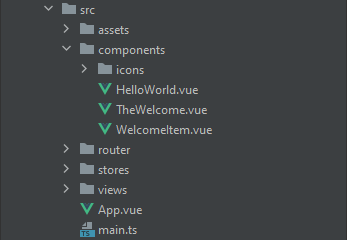
\includegraphics[width=0.4\textwidth]{img/vueFileStructure}
    \caption{Projektstruktur}
    \label{fig:vueProjektstruktur}
\end{figure}

\subsection*{Der virtuelle DOM}
Das Ändern des HTML-DOMs ist aufwändig und kann zu Performanceproblemen führen.
Für eine bessere Performance benutzt Vue.js einen virtuellen DOM.
Der virtuelle DOM ist eine Kopie des eigentlichen DOM.
Änderungen werden zunächst am virtuellen DOM vorgenommen.
Die Änderungen am virtuellen DOM ermöglicht es mehrere Änderungen zu bündeln,
bevor der reelle DOM angepasst wird. \cite[S. 10-11]{steyer2019} %TODO https://vuejs.org/guide/extras/rendering-mechanism.html#render-pipeline ?

\newpage

\subsection*{Model-View-ViewModel}
In Vue.js findet das MVVM-Pattern Anwendung.
Das sogenannte \emph{ViewModel} übernimmt die Vermittlung zwischen der View
und der Daten mit Businesslogik im Model.
Die Aufgabe des ViewModels übernimmt Vue.js.\cite[S. 43]{steyer2019}\footnote{In der Quelle ist die Rede von "MVVC". Aus dem Kontext ist klar, dass es sich um einen Tippfehler handelt und "MVVM" gemeint ist.}

\begin{figure}[H]
    \centering
    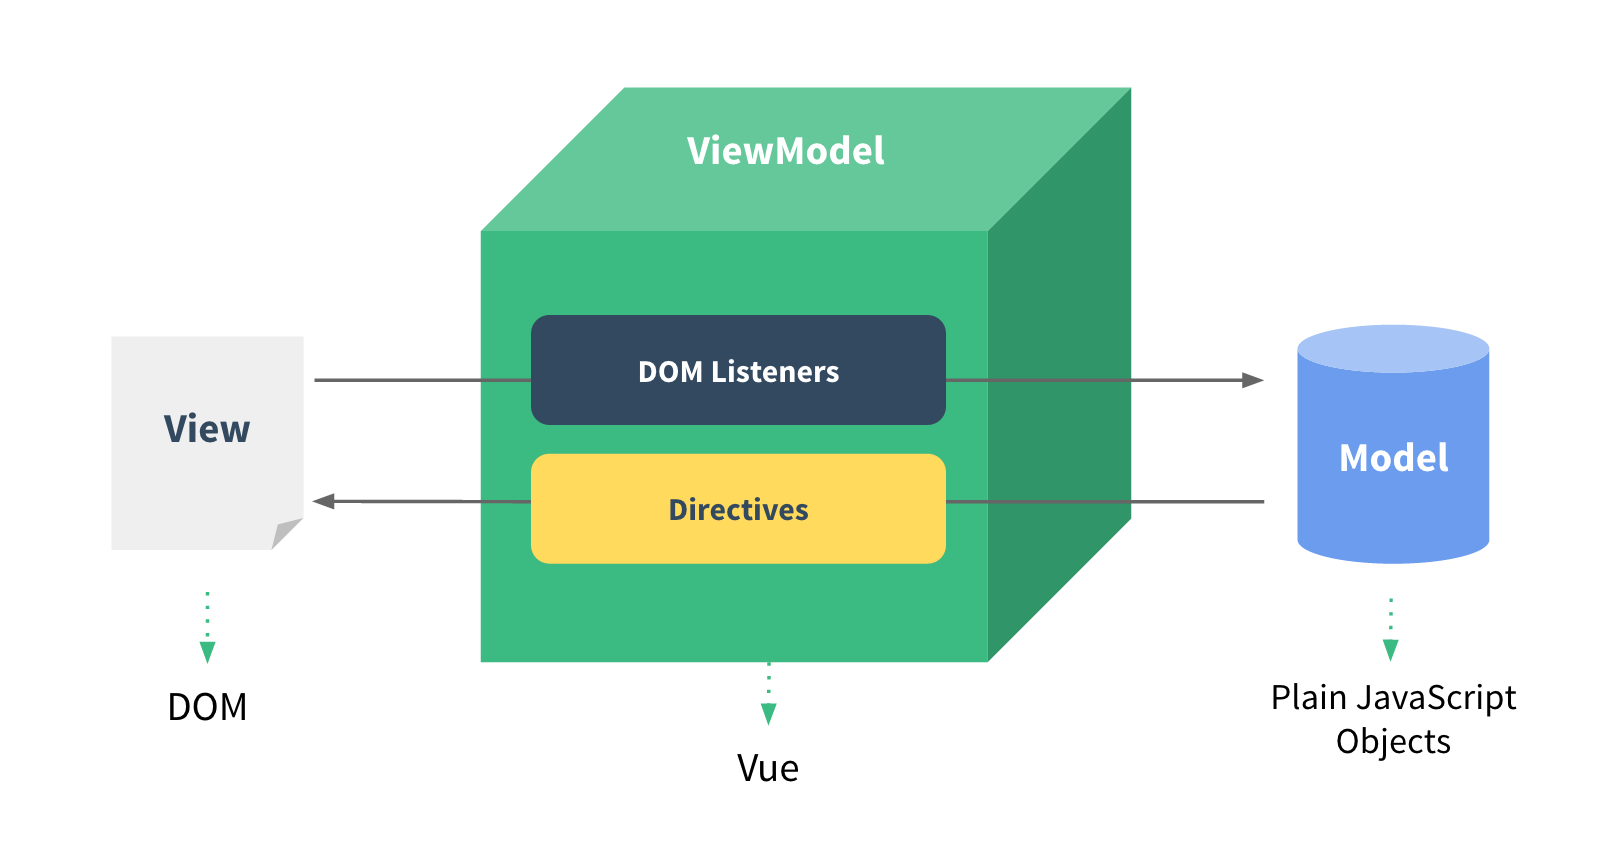
\includegraphics[width=0.8\textwidth]{img/mvvm}
    \caption{MVVM in Vue.js \cite{gettingStarted012}}
    \label{fig:mvvm}
\end{figure}

% ----------------------------------------------------------------------------
%! Author = biebl
%! Date = 12.05.2023


\chapter{Vergleich zu Angular anhand einer einfachen App}\label{ch:vergleich-zu-angular-anhand-einer-einfachen-app}


\section{Einführung in den Vergleich}
Für eine Gegenüberstellung mit Angular wurde jeweils in Vue.js und in Angular eine
simple Einkaufslistenapp erstellt.
Das Ziel war es, mit beiden Frameworks eine möglichst ähnliche Einkaufslistenapp zu entwickeln und
so von beiden Frameworks einen direkten Vergleich zu erstellen.
Die App besteht aus zwei Seiten: einer Checklisten-Seite und einer Seite zur Erstellung und Bearbeitung der Einträge.

Die Checklisten-Seite enthält eine Liste mit Mengenangaben der einzukaufenden Artikel und ermöglicht es dem Benutzer, die Artikel abzuhaken.
Auf der Bearbeiten-Seite können Artikel mit Mengenangaben erstellt, bearbeitet und gelöscht werden.
Für diese Gegenüberstellung wurde auf ein Backend und auf aufwändiges Design verzichtet.
Ein Screenshot der beiden Seiten (siehe Abbildung \ref{fig:checklistenseite} und \ref{fig:editlistenseite}) und die Links zu den GitHub Repositories der beiden Apps befinden sich im Anhang.


\section{Gegenüberstellung von Vue.js und Angular anhand einer einfachen App}
Zunächst wird auf die Ähnlichkeiten zwischen beiden Frameworks eingegangen, die beim Entwickeln der Einkaufslistenapp aufgefallen sind.
Beide Frameworks haben ähnliche Direktiven wie zum Beispiel \texttt{v-model} und \texttt{[(ngModel)]} oder \texttt{v-for} und \texttt{*ngFor},
die in ihrer Verwendung fast gleich sind.
Die beiden Frameworks ermöglichen unidirektionale Datenbindung mit der Mustache-Syntax.
Das Routing ist bei beiden Frameworks nicht standardmäßig vorhanden.
Bei Angular muss das Routing erst aktiviert werden, in Vue.js muss die Routing-Erweiterung installiert werden.
Die Verwendung des Routers ist bei beiden ähnlich.
Man legt den Pfad mit der zugehörigen Komponente in einem Array fest
und übergibt dies abschließend der App-Instanz.
Mit einem \texttt{<router-outlet>}-Tag in Angular oder einem \texttt{<RouterView>}-Tag in Vue.js wird dann angegeben, wo die aktuelle Route gerendert werden soll.
Sowohl Vue.js als auch Angular bieten bereits beim Erstellen des Projekts die Möglichkeit, das Routing zu ergänzen.
Während in Vue.js in der Regel mit SFC gearbeitet wird, besteht in Angular eine Komponente aus vier Dateien.
Die vier Dateien einer Angular Komponente unterteilen sich in eine TypeScript-, eine HTML-, eine Style- und einer Verwaltungsdatei.
In Vue.js legt man für eine neue Komponente eine neue \texttt{.vue}-Datei an,
in Angular erfolgt es über die Angular CLI, welche einen Ordner mit den vier Dateien generiert.
Für die Einkauflistenapp sollte der Inhalt der Liste zentral sein, damit sowohl von der Checklisten-Seite als auch von der Bearbeiten-Seite
auf die Einträge zugegriffen werden kann.
In Vue.js ist dies mit dem in Abschnitt \ref{sec:state-management-in-vue.js} erwähnten Pinia möglich.
Mit Pinia wurde eine Store für die Einkaufliste mit den darin enthaltenen Items erstellt.
Auf den Einkaufslisten-Store kann dann von der Checklisten-Seite und der Bearbeiten-Seite zugegriffen werden.
In Angular wurde es mit einem Service gelöst.
Der erstellte Service in Angular ermöglicht einen gleichwertigen zentralen Zugriff.
\\
Auffällig ist der Größenunterschied der beiden Projektordner.
Die Implementierung mit Vue.js hat 29 MB, dagegen hat die Implementierung mit Angular eine Größe von 370 MB.
Der Entwicklungsserver der Vue.js Implementierung braucht 127 MB Arbeitsspeicher, für den Entwicklungsserver der Angular Implementierung
werden 460 MB Arbeitsspeicher beansprucht.
Nach dem Build-Prozess beansprucht die Vue.js-Implementierung einen Speicherplatz von 88 KB und einen Arbeitsspeicher von 84 MB.
Die Angular-Implementierung erfordert nach dem Build-Prozess einen Speicherplatz von 287 KB und einen Arbeitsspeicher von 92 MB.

%\section{Vergleich zu React.js}
%Aufgrund des Umfangs der Arbeit verzichte ich beim Vergleich zu React.js auf eine solche Gegenüberstellung wie in Abschnitt \ref{sec:vergleich-zu-angular-und-gegenuberstellung-anhand-einer-einfachen-app}


%\section{Vor- und Nachteile}
%! Author = biebl
%! Date = 12.05.2023


\chapter{Fazit}
Die in Abschnitt \ref{sec:geschichte} von Evan You definierten Ziele für Vue.js sind meines erachtens erfüllt.
Die Absicht ein schlankes Framework zu erstellen ist erfüllt und wird deutlich beim Vergleichen der Speicherauslastung
der zwei äquivalenten Einkaufslistenapps.
Die Dynamik von Vue.js wird durch die Modulare erweiterbarkeit und meines erachtens durch das
Konzept der SFC deutlich.
Während ich in Angular immer wieder zwischen drei Dateien springen muss, um eine Komponente zu bearbeiten,
ist in Vue.js alles zentral in einer Datei.
Die ähnliche Umsetzung einiger Konzepte wie das Routing oder die Verwendung von Direktiven machen
den wechsel zwischen Angular und Vue.js einfacher.
Für kleinere Anwendungen ist für mich Vue.js aufgrund der bereits genannten Konzepte vorzuziehen.
Wie sich Vue.js im Vergleich zu Angular bei größeren Projekten schlägt, lässt sich aus dem Vergleich
in Abschnitt \ref{ch:vergleich-zu-angular-anhand-einer-einfachen-app} nicht eindeutig sagen.
Der Vergleich in Abschnitt \ref{ch:vergleich-zu-angular-anhand-einer-einfachen-app} ist für Rückschlüsse
auf umfangreichere Projekte ungeeignet, da eine Betrachtung von Aspekten wie zusammenspiel mit einem Backend
oder Betrachtung des Featureumfangs fehlen.
Der Vergleich in Abschnitt \ref{ch:vergleich-zu-angular-anhand-einer-einfachen-app} bringt viel mehr einen
Einblick von Vue.js für Leute die bereits Erfahrung mit Angular haben.
Abschließend kann ich sagen Vue.js ist das, was es sein möchte, eine schlankere Alternative zu Angular.

%! Author = biebl
%! Date = 12.05.2023

\chapter{Ausblick}
Man könnte noch einen passenderen Versuch finden, um zu testen,
wie sich Vue.js im Vergleich zu Angular bei größeren Projekten schlägt.
Des Weiteren könnte man noch einen Vergleich zu React.js ziehen,
mit einer ähnlichen Methode wie in Abschnitt \ref{ch:vergleich-zu-angular-anhand-einer-einfachen-app}.
Darüber hinaus bietet Vue.js weiter Features die aufgrund der Kürze der Arbeit keine erwähnung fanden.
Features, die man noch betrachten könnte, wären Teleport, Serverseitigesrendern, Form Validation und vieles mehr.
Was in dieser Arbeit nicht betrachtet wurde, sind UI Frameworks wie Vuetify\footnote{\url{https://vuetifyjs.com/en/}} in verbindung mit Vue.js.
Der Support für Vue 2 endet am 31. Dezember 2023 \cite{vueFAQ}.
Weitere Pläne für Vue.js könnten auf der vom 24. bis 26. Mai stattfinden VueConfUS\footnote{\url{http://vueconf.us/}} bekannt werden.
%% ----------------------------------------------------------------------------
% Copyright (c) 2016 - 2020 by Burkhardt Renz. All rights reserved.
% Die Vorlage für eine Abschlussarbeit in der Informatik am Fachbereich
% MNI der THM ist lizenziert unter einer Creative Commons
% Namensnennung-Nicht kommerziell 4.0 International Lizenz.
%
% Id:$
% ----------------------------------------------------------------------------

\chapter{Was ist \LaTeX\ und wie ist eine \LaTeX-Datei aufgebaut?}

Der Text dieses Kapitals steht in der Datei \verb=aufbau.tex=. Die
Erläuterungen ab Abschnitt \ref{sec:aufbau} beziehen sich auf die Datei
\verb=vorlage.tex=.

\section{Etwas Geschichte -- oder ein paar Geschichten}

Die ersten Bände von \emph{The Art of Computer Programming}
(\textsc{TAOCP}) von Donald Knuth wurden im Bleisatz gesetzt. In den
1970er Jahren aber starb der Bleisatz aus und wurde durch den Fotosatz
ersetzt. Knuth war mit den damaligen Fotosatz-Systemen sehr unzufrieden,
weil sie mathematische Formeln nicht gut darstellen konnten. Das brachte
ihn auf die Idee selbst ein Satzsystem zu entwickeln, das für
Texte der Mathematik und Informatik typografisch hochwertige Ergebnisse
erreichen sollte. Zunächst dachte er, ein solches Programm könne in
einem Jahr oder so erstellt werden. Es dauerte dann doch etwa
länger -- siehe Tabelle \ref{tbl:geschichte}.\footnote{ Die Entwicklung
von \TeX\ ist auch ein interessanter Fall von Software-Engineering,
siehe Donald E. Knuth \emph{The Errors of \TeX} in: Tom de Marco und
Timothy Lister (Hrsg.) \emph{Software State-of-the-Art: Selected
Papers} New York NY: Dorste Publishing House, 1990.}

Knuths Idee \cite{knuth99} bestand darin, dass Text, Formeln und Layout
gewissermaßen programmiert werden. Das Satzsystem konsumiert ein solches
\enquote{Programm} und macht daraus ein Dokument --- heutzutage in der
Regel ein PDF-Dokument. Das System sollte natürlich erweiterbar und
anpassbar sein, weshalb die Sprache, die Knuth entwickelt hat, im Grunde
eine Makrosprache ist und es deshalb auch erlaubt eigene Befehle zu
schreiben. Knuth hat einen Satz an Makros entwickelt, den man
\textsc{Plain}\kern2pt\TeX\ nennt -- diese Makros sind sehr nahe am Kern
von \TeX, \emph{low level} sozusagen.

Leslie Lamport\footnote{ Leslie Lamport hat wichtige Beiträge zur
Theorie verteilter Systeme geleistet.} hat eine Menge von Makros
entwickelt, die auf \TeX\ aufbauen und das Setzen von Büchern, Berichten
und Artikeln erheblich vereinfachen. Diese Makros nannte er \LaTeX\
\cite{lamport94}.  Leslie Lamport erzählt über die Entstehung  von
\LaTeX\
(\url{http://research.microsoft.com/en-us/um/people/lamport/pubs/pubs.html#latex}):

\begin{quote}
In the early 80s, I was planning to write the Great American Concurrency
Book.  I was a \TeX\ user, so I would need a set of macros.  I thought
that, with a little extra effort, I could make my macros usable by
others.  Don Knuth had begun issuing early releases of the current
version of \TeX, and I figured I could write what would become its
standard macro package.  That was the beginning of \LaTeX. 	\\
\dots\\
Meanwhile, I still haven't written the Great American Concurrency
Book.
\end{quote}

\LaTeX\ trennt im Grunde die Befehle, die den Inhalt und die Struktur
eines Texts betreffen von den Befehlen, die für die typografische
Gestaltung sorgen.  \LaTeX\ stellt eine Reihe von sogenannten
Dokumentklassen bereit, die das Layout von Artikeln, Berichten, Büchern
und Briefen bereits enthalten, so dass man sich beim Schreiben nicht
mehr darum kümmern muss.

Die Dokumentklassen von \LaTeX\ erzeugen eine Typografie, die an
amerikanischen Konventionen orientiert ist. \textsf{KOMA-Script} ist eine
Sammlung von Dokumentklassen, die sich an europäischer Typografie
orientieren. Frank Neukam entwickelte Anfang der 1990er Jahr
\textsf{Script}, das Markus Kohm zu \textsf{KOMA-Script}
weiterentwickelte \cite{koma16}. Wir verwenden für die Vorlage die
Dokumentklasse von \textsf{KOMA-Script} für das Setzen von Büchern.

\section{Der Aufbau einer \LaTeX-Datei}
\label{sec:aufbau}

Eine \LaTeX-Datei beginnt mit der Angabe der Dokumentklasse mitsamt
ihren Optionen. Darauf folgt die sogenannte Präambel, in der benötigte
Pakete angegeben, Einstellungen festgelegt und auch eigene Makros
definiert werden. Darauf folgt in der Umgebung \verb=document= der
eigentliche Text.

\subsection{Dokumentklasse}

Wir verwenden für die Abschlussarbeit die Dokumentklasse \verb=scrbook=
von \textsf{KOMA-Script}. Diese Dokumentklasse ist vorgesehen für den
Satz von Büchern und sorgt dafür, dass Kapitel immer auf einer rechten
(also vorderen) Seite beginnen.

Die Dokumentklasse hat in der Regel geeignete Voreinstellungen für eine
Abschlussarbeit. Deshalb ändern wir nur einige wenige der Optionen von
\verb=scrbook=. In \cite{partosch15} werden weitere Optionen erläutert.

\subsection{Präambel}

In der Präambel binden wir benötigte Pakete ein.  Pakete sind
vorgefertigte Sammlungen von Makros für \LaTeX. Es  gibt für nahezu jede
denkbare Aufgabe solche Pakete, die man im \TeX\ Catalogue
\url{http://texcatalogue.ctan.org} finden kann.

Unsere Vorlage bindet die wichtigsten und für eine Arbeit im Feld der
Informatik in der Regel benötigten Pakete ein. Auch hierzu findet man
weitere Informationen in \cite{partosch15}.

Darüber hinaus stehen Einstellungen in der Präambel, bei uns z.B. zur
Nummerierungstiefe.

Eigene Makros kann man auch in der Präambel unterbringen.

\subsection{Die Umgebung \texttt{document}}

Nach der Präambel kommt die Umgebung \verb=document=. In \LaTeX\ nennt
man Blöcke, die durch \verb=\begin{umgebung}= und \verb=\end{umgebung}=
begrenzt sind \emph{Umgebung}. In der Regel werden zu Beginn der
Umgebung bestimmte Einstellungen ein- und am Ende der Umgebung wieder
ausgeschaltet.

Der eigentliche Text der Arbeit steht also in der Klammer

\begin{lstlisting}
\begin{document}

% hierher kommt der eigentliche Text

\end{document}
\end{lstlisting}


Es ist ratsam, den eigentlichen Text in verschiedene Dateien zu
verteilen, etwa pro Kapitel eine Datei. Diese Dateien können dann in die
führende Datei eingebunden werden, bei uns durch folgende Befehle:

\begin{lstlisting}

% ----------------------------------------------------------------------------
% Copyright (c) 2016 - 2020 by Burkhardt Renz. All rights reserved.
% Die Vorlage für eine Abschlussarbeit in der Informatik am Fachbereich
% MNI der THM ist lizenziert unter einer Creative Commons
% Namensnennung-Nicht kommerziell 4.0 International Lizenz.
%
% Id:$
% ----------------------------------------------------------------------------

\chapter{Was ist \LaTeX\ und wie ist eine \LaTeX-Datei aufgebaut?}

Der Text dieses Kapitals steht in der Datei \verb=aufbau.tex=. Die
Erläuterungen ab Abschnitt \ref{sec:aufbau} beziehen sich auf die Datei
\verb=vorlage.tex=.

\section{Etwas Geschichte -- oder ein paar Geschichten}

Die ersten Bände von \emph{The Art of Computer Programming}
(\textsc{TAOCP}) von Donald Knuth wurden im Bleisatz gesetzt. In den
1970er Jahren aber starb der Bleisatz aus und wurde durch den Fotosatz
ersetzt. Knuth war mit den damaligen Fotosatz-Systemen sehr unzufrieden,
weil sie mathematische Formeln nicht gut darstellen konnten. Das brachte
ihn auf die Idee selbst ein Satzsystem zu entwickeln, das für
Texte der Mathematik und Informatik typografisch hochwertige Ergebnisse
erreichen sollte. Zunächst dachte er, ein solches Programm könne in
einem Jahr oder so erstellt werden. Es dauerte dann doch etwa
länger -- siehe Tabelle \ref{tbl:geschichte}.\footnote{ Die Entwicklung
von \TeX\ ist auch ein interessanter Fall von Software-Engineering,
siehe Donald E. Knuth \emph{The Errors of \TeX} in: Tom de Marco und
Timothy Lister (Hrsg.) \emph{Software State-of-the-Art: Selected
Papers} New York NY: Dorste Publishing House, 1990.}

Knuths Idee \cite{knuth99} bestand darin, dass Text, Formeln und Layout
gewissermaßen programmiert werden. Das Satzsystem konsumiert ein solches
\enquote{Programm} und macht daraus ein Dokument --- heutzutage in der
Regel ein PDF-Dokument. Das System sollte natürlich erweiterbar und
anpassbar sein, weshalb die Sprache, die Knuth entwickelt hat, im Grunde
eine Makrosprache ist und es deshalb auch erlaubt eigene Befehle zu
schreiben. Knuth hat einen Satz an Makros entwickelt, den man
\textsc{Plain}\kern2pt\TeX\ nennt -- diese Makros sind sehr nahe am Kern
von \TeX, \emph{low level} sozusagen.

Leslie Lamport\footnote{ Leslie Lamport hat wichtige Beiträge zur
Theorie verteilter Systeme geleistet.} hat eine Menge von Makros
entwickelt, die auf \TeX\ aufbauen und das Setzen von Büchern, Berichten
und Artikeln erheblich vereinfachen. Diese Makros nannte er \LaTeX\
\cite{lamport94}.  Leslie Lamport erzählt über die Entstehung  von
\LaTeX\
(\url{http://research.microsoft.com/en-us/um/people/lamport/pubs/pubs.html#latex}):

\begin{quote}
In the early 80s, I was planning to write the Great American Concurrency
Book.  I was a \TeX\ user, so I would need a set of macros.  I thought
that, with a little extra effort, I could make my macros usable by
others.  Don Knuth had begun issuing early releases of the current
version of \TeX, and I figured I could write what would become its
standard macro package.  That was the beginning of \LaTeX. 	\\
\dots\\
Meanwhile, I still haven't written the Great American Concurrency
Book.
\end{quote}

\LaTeX\ trennt im Grunde die Befehle, die den Inhalt und die Struktur
eines Texts betreffen von den Befehlen, die für die typografische
Gestaltung sorgen.  \LaTeX\ stellt eine Reihe von sogenannten
Dokumentklassen bereit, die das Layout von Artikeln, Berichten, Büchern
und Briefen bereits enthalten, so dass man sich beim Schreiben nicht
mehr darum kümmern muss.

Die Dokumentklassen von \LaTeX\ erzeugen eine Typografie, die an
amerikanischen Konventionen orientiert ist. \textsf{KOMA-Script} ist eine
Sammlung von Dokumentklassen, die sich an europäischer Typografie
orientieren. Frank Neukam entwickelte Anfang der 1990er Jahr
\textsf{Script}, das Markus Kohm zu \textsf{KOMA-Script}
weiterentwickelte \cite{koma16}. Wir verwenden für die Vorlage die
Dokumentklasse von \textsf{KOMA-Script} für das Setzen von Büchern.

\section{Der Aufbau einer \LaTeX-Datei}
\label{sec:aufbau}

Eine \LaTeX-Datei beginnt mit der Angabe der Dokumentklasse mitsamt
ihren Optionen. Darauf folgt die sogenannte Präambel, in der benötigte
Pakete angegeben, Einstellungen festgelegt und auch eigene Makros
definiert werden. Darauf folgt in der Umgebung \verb=document= der
eigentliche Text.

\subsection{Dokumentklasse}

Wir verwenden für die Abschlussarbeit die Dokumentklasse \verb=scrbook=
von \textsf{KOMA-Script}. Diese Dokumentklasse ist vorgesehen für den
Satz von Büchern und sorgt dafür, dass Kapitel immer auf einer rechten
(also vorderen) Seite beginnen.

Die Dokumentklasse hat in der Regel geeignete Voreinstellungen für eine
Abschlussarbeit. Deshalb ändern wir nur einige wenige der Optionen von
\verb=scrbook=. In \cite{partosch15} werden weitere Optionen erläutert.

\subsection{Präambel}

In der Präambel binden wir benötigte Pakete ein.  Pakete sind
vorgefertigte Sammlungen von Makros für \LaTeX. Es  gibt für nahezu jede
denkbare Aufgabe solche Pakete, die man im \TeX\ Catalogue
\url{http://texcatalogue.ctan.org} finden kann.

Unsere Vorlage bindet die wichtigsten und für eine Arbeit im Feld der
Informatik in der Regel benötigten Pakete ein. Auch hierzu findet man
weitere Informationen in \cite{partosch15}.

Darüber hinaus stehen Einstellungen in der Präambel, bei uns z.B. zur
Nummerierungstiefe.

Eigene Makros kann man auch in der Präambel unterbringen.

\subsection{Die Umgebung \texttt{document}}

Nach der Präambel kommt die Umgebung \verb=document=. In \LaTeX\ nennt
man Blöcke, die durch \verb=\begin{umgebung}= und \verb=\end{umgebung}=
begrenzt sind \emph{Umgebung}. In der Regel werden zu Beginn der
Umgebung bestimmte Einstellungen ein- und am Ende der Umgebung wieder
ausgeschaltet.

Der eigentliche Text der Arbeit steht also in der Klammer

\begin{lstlisting}
\begin{document}

% hierher kommt der eigentliche Text

\end{document}
\end{lstlisting}


Es ist ratsam, den eigentlichen Text in verschiedene Dateien zu
verteilen, etwa pro Kapitel eine Datei. Diese Dateien können dann in die
führende Datei eingebunden werden, bei uns durch folgende Befehle:

\begin{lstlisting}

% ----------------------------------------------------------------------------
% Copyright (c) 2016 - 2020 by Burkhardt Renz. All rights reserved.
% Die Vorlage für eine Abschlussarbeit in der Informatik am Fachbereich
% MNI der THM ist lizenziert unter einer Creative Commons
% Namensnennung-Nicht kommerziell 4.0 International Lizenz.
%
% Id:$
% ----------------------------------------------------------------------------

\chapter{Was ist \LaTeX\ und wie ist eine \LaTeX-Datei aufgebaut?}

Der Text dieses Kapitals steht in der Datei \verb=aufbau.tex=. Die
Erläuterungen ab Abschnitt \ref{sec:aufbau} beziehen sich auf die Datei
\verb=vorlage.tex=.

\section{Etwas Geschichte -- oder ein paar Geschichten}

Die ersten Bände von \emph{The Art of Computer Programming}
(\textsc{TAOCP}) von Donald Knuth wurden im Bleisatz gesetzt. In den
1970er Jahren aber starb der Bleisatz aus und wurde durch den Fotosatz
ersetzt. Knuth war mit den damaligen Fotosatz-Systemen sehr unzufrieden,
weil sie mathematische Formeln nicht gut darstellen konnten. Das brachte
ihn auf die Idee selbst ein Satzsystem zu entwickeln, das für
Texte der Mathematik und Informatik typografisch hochwertige Ergebnisse
erreichen sollte. Zunächst dachte er, ein solches Programm könne in
einem Jahr oder so erstellt werden. Es dauerte dann doch etwa
länger -- siehe Tabelle \ref{tbl:geschichte}.\footnote{ Die Entwicklung
von \TeX\ ist auch ein interessanter Fall von Software-Engineering,
siehe Donald E. Knuth \emph{The Errors of \TeX} in: Tom de Marco und
Timothy Lister (Hrsg.) \emph{Software State-of-the-Art: Selected
Papers} New York NY: Dorste Publishing House, 1990.}

Knuths Idee \cite{knuth99} bestand darin, dass Text, Formeln und Layout
gewissermaßen programmiert werden. Das Satzsystem konsumiert ein solches
\enquote{Programm} und macht daraus ein Dokument --- heutzutage in der
Regel ein PDF-Dokument. Das System sollte natürlich erweiterbar und
anpassbar sein, weshalb die Sprache, die Knuth entwickelt hat, im Grunde
eine Makrosprache ist und es deshalb auch erlaubt eigene Befehle zu
schreiben. Knuth hat einen Satz an Makros entwickelt, den man
\textsc{Plain}\kern2pt\TeX\ nennt -- diese Makros sind sehr nahe am Kern
von \TeX, \emph{low level} sozusagen.

Leslie Lamport\footnote{ Leslie Lamport hat wichtige Beiträge zur
Theorie verteilter Systeme geleistet.} hat eine Menge von Makros
entwickelt, die auf \TeX\ aufbauen und das Setzen von Büchern, Berichten
und Artikeln erheblich vereinfachen. Diese Makros nannte er \LaTeX\
\cite{lamport94}.  Leslie Lamport erzählt über die Entstehung  von
\LaTeX\
(\url{http://research.microsoft.com/en-us/um/people/lamport/pubs/pubs.html#latex}):

\begin{quote}
In the early 80s, I was planning to write the Great American Concurrency
Book.  I was a \TeX\ user, so I would need a set of macros.  I thought
that, with a little extra effort, I could make my macros usable by
others.  Don Knuth had begun issuing early releases of the current
version of \TeX, and I figured I could write what would become its
standard macro package.  That was the beginning of \LaTeX. 	\\
\dots\\
Meanwhile, I still haven't written the Great American Concurrency
Book.
\end{quote}

\LaTeX\ trennt im Grunde die Befehle, die den Inhalt und die Struktur
eines Texts betreffen von den Befehlen, die für die typografische
Gestaltung sorgen.  \LaTeX\ stellt eine Reihe von sogenannten
Dokumentklassen bereit, die das Layout von Artikeln, Berichten, Büchern
und Briefen bereits enthalten, so dass man sich beim Schreiben nicht
mehr darum kümmern muss.

Die Dokumentklassen von \LaTeX\ erzeugen eine Typografie, die an
amerikanischen Konventionen orientiert ist. \textsf{KOMA-Script} ist eine
Sammlung von Dokumentklassen, die sich an europäischer Typografie
orientieren. Frank Neukam entwickelte Anfang der 1990er Jahr
\textsf{Script}, das Markus Kohm zu \textsf{KOMA-Script}
weiterentwickelte \cite{koma16}. Wir verwenden für die Vorlage die
Dokumentklasse von \textsf{KOMA-Script} für das Setzen von Büchern.

\section{Der Aufbau einer \LaTeX-Datei}
\label{sec:aufbau}

Eine \LaTeX-Datei beginnt mit der Angabe der Dokumentklasse mitsamt
ihren Optionen. Darauf folgt die sogenannte Präambel, in der benötigte
Pakete angegeben, Einstellungen festgelegt und auch eigene Makros
definiert werden. Darauf folgt in der Umgebung \verb=document= der
eigentliche Text.

\subsection{Dokumentklasse}

Wir verwenden für die Abschlussarbeit die Dokumentklasse \verb=scrbook=
von \textsf{KOMA-Script}. Diese Dokumentklasse ist vorgesehen für den
Satz von Büchern und sorgt dafür, dass Kapitel immer auf einer rechten
(also vorderen) Seite beginnen.

Die Dokumentklasse hat in der Regel geeignete Voreinstellungen für eine
Abschlussarbeit. Deshalb ändern wir nur einige wenige der Optionen von
\verb=scrbook=. In \cite{partosch15} werden weitere Optionen erläutert.

\subsection{Präambel}

In der Präambel binden wir benötigte Pakete ein.  Pakete sind
vorgefertigte Sammlungen von Makros für \LaTeX. Es  gibt für nahezu jede
denkbare Aufgabe solche Pakete, die man im \TeX\ Catalogue
\url{http://texcatalogue.ctan.org} finden kann.

Unsere Vorlage bindet die wichtigsten und für eine Arbeit im Feld der
Informatik in der Regel benötigten Pakete ein. Auch hierzu findet man
weitere Informationen in \cite{partosch15}.

Darüber hinaus stehen Einstellungen in der Präambel, bei uns z.B. zur
Nummerierungstiefe.

Eigene Makros kann man auch in der Präambel unterbringen.

\subsection{Die Umgebung \texttt{document}}

Nach der Präambel kommt die Umgebung \verb=document=. In \LaTeX\ nennt
man Blöcke, die durch \verb=\begin{umgebung}= und \verb=\end{umgebung}=
begrenzt sind \emph{Umgebung}. In der Regel werden zu Beginn der
Umgebung bestimmte Einstellungen ein- und am Ende der Umgebung wieder
ausgeschaltet.

Der eigentliche Text der Arbeit steht also in der Klammer

\begin{lstlisting}
\begin{document}

% hierher kommt der eigentliche Text

\end{document}
\end{lstlisting}


Es ist ratsam, den eigentlichen Text in verschiedene Dateien zu
verteilen, etwa pro Kapitel eine Datei. Diese Dateien können dann in die
führende Datei eingebunden werden, bei uns durch folgende Befehle:

\begin{lstlisting}

\input{aufbau}      % Kapitel 1
\input{gliederung}  % Kapitel 2
\input{elemente}    % Kapitel 3

\end{lstlisting}

% ----------------------------------------------------------------------------
      % Kapitel 1
% ----------------------------------------------------------------------------
% Copyright (c) 2016 -2020 by Burkhardt Renz. All rights reserved.
% Die Vorlage für eine Abschlussarbeit in der Informatik am Fachbereich
% MNI der THM ist lizenziert unter einer Creative Commons
% Namensnennung-Nicht kommerziell 4.0 International Lizenz.
%
% Id:$
% ----------------------------------------------------------------------------

\chapter{Elemente für die Gliederung}

Der Text dieses Kapitels steht in \verb=gliederung.tex=. Er bezieht sich
auf \verb=vorlage.tex= und \verb=gliederung.tex=.

\section{Teile}

Eine Abschlussarbeit besteht aus drei großen Teilen:

\begin{itemize}
	\item Dem Vorderteil (\verb=frontmatter=) mit
		\begin{itemize}
			\item der Titelseite,
			\item der eidesstattlichen Erklärung,
			\item der Zusammenfassung,
			\item dem Inhaltsverzeichnis und
			\item den Verzeichnissen von Abbildungen, Tabellen und Listings,
		\end{itemize}
	\item dem Hauptteil (\verb=mainmatter=) mit den Kapiteln der Arbeit
		und
	\item dem Anhang (\verb=backmatter=) mit Anhängen und dem
		Literaturverzeichnis	
\end{itemize}

Manchmal erwarten Dozentinnen oder Dozenten, dass eine Abschlussarbeit
Verzeichnisse der Abbildungen, Tabellen und Listings oder auch ein Glossar
der verwendeten Begriffe enthält. Deshalb enthält unsere Vorlage diese
Verzeichnisse. Ein Glossar kann man mit der Umgebung \verb=description=
oder \verb=labeling= erzeugen, die in Abschnitt
\ref{sec:stichwortlisten}  beschrieben werden.

Ich persönlich finde, dass man auf diese Verzeichnisse verzichten kann.
Und ein Glossar ist meines Erachtens nur nötig, wenn man viele
Fachbegriffe in der Arbeit verwendet, die einem in der Informatik
Kundigen nicht geläufig sind.

\section{Kapitel und ihre Untergliederungen}

Die Dokumentklasse \verb=scrbook= hat als Möglichkeiten der Gliederung
zunächst den Teil (\verb=part=). Er wird in diesem Dokument nicht
verwendet und meistens ist eine Bachelor- oder Masterarbeit nicht so
umfangreich, als dass man sie in Teile unterteilen müsste.

Die nächste Ebene ist das Kapital (\verb=chapter=), wie wir auf der
vorigen Seite den Anfang eines solchen sehen. Kapitel beginnen immer auf
einer rechten Seite.

Dann kommt der Abschnitt (\verb=section=) --- in einem solchen befinden wir
uns im Moment.

\subsection{Unterabschnitt}

Dies ist eine \verb=subsection=.

\subsubsection{Unterunterabschnitt}

Jetzt sind wir noch eine Ebene tiefer, in der \verb=subsubsection=. Eine
Gliederung sollte ausgewogen sein, auch in Bezug auf die
Gliederungstiefe. Deshalb sollte man eher nicht bis zum
Unterunterabschnitt gehen.


\paragraph{Absatz mit Überschrift}

Dies ist ein Absatz mit Überschrift \verb=paragraph=. Die Überschrift
wird im Dokument hervorgehoben, hat aber keine eigene Zeile. Typografen
nennen das auch einen \enquote{Spieß}.

\subparagraph{Unterabsatz}

Dies ist ein Unterabsatz \verb=subparagraph=, auch ein \enquote{Spieß}.

\section{Untergliederungen im Text}

\subsection{Aufzählungen}

Man kann nummerierte Aufzählungen mit der Umgebung \verb=enumerate=
erzeugen. Dies eignet sich für Aufzählungen, die eine Reihenfolge haben
und ist oft einer Aneinanderreihung im Text vorzuziehen, weil
übersichtlicher.

Eine Bachelorarbeit besteht aus

\begin{enumerate}
	\item einem ersten Kapitel
		\begin{enumerate}
			\item einem ersten Abschnitt darin,
			\item einem zweiten Abschnitt darin,
		\end{enumerate}
	\item einem zweiten Kapitel
	\item usw. usf.	
\end{enumerate}

Aufzählungen, die keine inhaltliche Reihenfolge haben, kann man mit der
Umgebung \verb=itemize= darstellen:

\begin{itemize}
	\item eine wichtige Aussage
	\item noch eine wichtige Aussage
		\begin{itemize}
			\item mit einer Ausprägung
			\item und noch einer Ausprägung	
		\end{itemize}
	\item \dots
\end{itemize}

\subsection{Stichwortlisten}
\label{sec:stichwortlisten}

Ein Beispiel für die Umgebung \verb=description= habe ich aus der
Dokumentation von \textsf{KOMA-Script} übernommen:

\begin{description}
	\item[empty] ist der Seitenstil, bei dem Kopf- und Fußzeile vollständig 
		leer bleiben. 
	\item[plain] ist der Seitenstil, bei dem keinerlei Kolumnentitel verwendet wird. 
	\item[headings] ist der Seitenstil für automatische Kolumnentitel. 
	\item[myheadings] ist der Seitenstil für manuelle Kolumnentitel. 
\end{description}

Es gibt auch noch die Umgebung \verb=labeling=, bei der man durch ein
Muster angeben kann, wie breit die Einrückung ist. Im Beispiel mit den
Seitenstilen könnte man das so machen:

\setkomafont{labelinglabel}{\sffamily\bfseries}
\begin{labeling}{myheadings}
	\item[empty] ist der Seitenstil, bei dem Kopf- und Fußzeile vollständig 
		leer bleiben. 
	\item[plain] ist der Seitenstil, bei dem keinerlei Kolumnentitel verwendet wird. 
	\item[headings] ist der Seitenstil für automatische Kolumnentitel. 
	\item[myheadings] ist der Seitenstil für manuelle Kolumnentitel. 
\end{labeling}

\section{Zum Literaturverzeichnis}

In der Vorlage findet man das Literaturverzeichnis in der Datei
\verb=litverz.tex=. 

Das Literaturverzeichnis kann man in \LaTeX\ auf zwei Arten erstellen:

Die einfache Variante besteht darin, dass man die Umgebung
\verb=bibliography= verwendet. So haben wir das in diesem Dokument
gemacht. Die Angaben zur Literatur stehen in \verb=litverz=. Jeder
Eintrag hat einen \emph{key}, den wir im Text im Befehl \verb=\cite=
referenzieren können. Die Referenz wird dann als Nummer im Text
angegeben und die entsprechende Nummer erscheint auch im
Literaturverzeichnis.

Die etwas aufwändigere Variante besteht darin, \verb=bibtex= zu
verwenden. Dies lohnt sich insbesondere dann, wenn man in verschiedenen
Manuskripte immer wieder dieselben Literaturverweise verwendet.

Mit \verb=bibtex= speichert man die Literaturangaben in einer Art
Datenbank, einer BibTeX-Datei. Die im Manuskript referenzierten Arbeiten
werden dann von \verb=bibtex= automatisch in das Literaturverzeichnis
übernommen. Die Formatierung des Verweises im Text und der Einträge im
Literaturverzeichnis wird dabei durch eine eigene Datei, dem
BibTeX-Stil, gesteuert. Will man die Verweise durch Nummern, wählt man
als Stil \verb=plain=, will man die Verweise durch die Abkürzung des
Autorennamens mit Angabe des Jahres, wählt man z.B. den Stil
\verb=alpha=. Es gibt eine Vielzahl solcher BibTeX-Stile, siehe
\url{https://www.ctan.org/tex-archive/biblio/bibtex/contrib}. Man kann sogar
eigene BibTeX-Stile definieren mit \verb=tex makebst=.

Mehr über BibTeX findet man z.B. bei \url{https://de.wikibooks.org/wiki/LaTeX-Kompendium:_Zitieren_mit_BibTeX}.

% ----------------------------------------------------------------------------
  % Kapitel 2
% ----------------------------------------------------------------------------
% Copyright (c) 2016 - 2020 by Burkhardt Renz. All rights reserved.
% Die Vorlage für eine Abschlussarbeit in der Informatik am Fachbereich
% MNI der THM ist lizenziert unter einer Creative Commons
% Namensnennung-Nicht kommerziell 4.0 International Lizenz.
%
% Id:$
% ----------------------------------------------------------------------------

\chapter{Elemente im Text}

Der Text dieses Kapitels steht in \verb=elemente.tex= und bezieht auch
auf diese Datei.

\section{Typografische Elemente}

Im laufenden Text kann man alles Mögliche machen. Gute Typografie geht
mit diesen Möglichkeiten sparsam um. Was in Texten der Informatik oft
vorkommt ist die \emph{Hervorhebung} mit dem Befehl \verb=\emph=. Man
verwendet kursive Schrift auch für fremdsprachige Worte im Text, etwa
\textit{digital typography}.
Für Schlüsselworte, Befehle der Kommandozeile u.ä. nimmt man gerne einen
passenden Zeichensatz, etwa \texttt{make vorlage.pdf}. 

Das Paket \verb=csquotes= sorgt dafür dass Anführungszeichen
typografisch korrekt verwendet werden. Im Deutschen werden die
\enquote{Gänsefüßchen} nämlich anders als die angelsächsischen
\foreignquote{english}{quotation marks} gesetzt.

Mehr über das Setzen von Text findet man in \cite{lkurz15}.

\section{Referenzen und Links}

Verweise auf die Literatur macht man mit dem Befehl \verb=\cite=.
Braucht man Querverweise auf Abschnitte im Text oder Abbildungen etc.,
so versieht man das Verweisziel mit einem \verb=\label= und verweist
dann mit \verb=\ref= oder \verb=\pageref=. Mehr dazu in
\cite[S.50]{partosch15}.

Links auf Quellen im Internet werden durch den Befehl \verb=\url=
angegeben und dadurch in PDF \enquote{anklickbar}, etwa wie
\url{https://tug.org/mactex/src/WelcomeToMacTeX.pdf}.

\section{Abbildungen}

\begin{figure}[!htb]
	\centering
	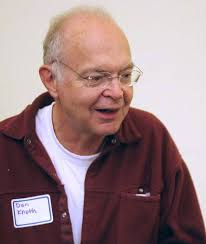
\includegraphics[width=.4\textwidth]{img/knuth.jpg}
	\caption{Donald Knuth}
	\label{fig:knuth}
\end{figure}


\begin{figure}[!htb]
	\centering
	\includegraphics[width=.4\textwidth]{img/783px-Test-Logo.svg}
	\caption{Test}
	\label{fig:test}
\end{figure}

Abbildungen bindet man mit \verb=\includegraphics= in einer Umgebung
\verb=figure= ein.
Man kann dann im Text auf die Abbildung \ref{fig:knuth} verweisen.
Man muss beachten, dass die Abbildung in einer sogenannten
\enquote{fließenden} Umgebung eingebunden wird, d.h. beim Setzen des
Dokuments bestimmt \TeX, an welcher Stelle genau im Dokument die
Abbildung erscheint.

Wie man an diesem Beispiel sieht, kann man beliebige Abbildungen etwa
\verb=jpg= wie in diesem Beispiel, aber auch \verb=pdf= einbinden. Man
kann also Abbildungen mit einem Grafikprogramm erstellen, als
\verb=pdf= speichern und dann einbinden.

\newcommand{\tikz}{Ti\emph{k}Z}

Es gibt aber auch \tikz\ (= \tikz\ ist kein Zeichenprogramm), das der
deutsche Informatiker Till Tantau entwickelt hat. Damit ist es möglich,
Abbildungen zu \enquote{programmieren}. Die Projektseite von \tikz\ ist
\url{https://sourceforge.net/projects/pgf/}. Interessant sind auch
die Beispiele auf \url{http://www.texample.net/tikz/examples/}.

\section{Tabellen}

Tabellen werden in einer \enquote{fließenden} Umgebung namens
\verb=table= eingegeben. Der eigentliche Inhalt der Tabelle kommt in die
Umgebung \verb=tabular=.

\begin{table}[!htb]
	\centering
	\caption{Die Geschichte von \TeX\ und \LaTeX}
	\begin{tabular}{ r p{13cm}}
		\toprule
		Jahr & Entwicklung\\
		\midrule
		1977 & Donald Knuth beginnt mit der Entwicklung von \TeX.\\
		1985 & \LaTeX\ (mächtige Makros, die die Verwendung von \TeX\
			vereinfachen, in dem sie Struktur und Layout trennen) wird von
			Leslie Lamport in der Version 2.09 freigegeben.\\
		1986 & Feier der Fertigstellung von \TeX\ im Computer Museum in
		Boston\\
		1986 & Leslie Lamport veröffentlicht \emph{\LaTeX: A Document
			Preparation System}.\\
		1993 & \LaTeXe\\
		2000 & pdf\TeX\ (entwickelt von Hàn Thé Thành)\\
			?  & Nach dem Tod von Donald Knuth bekommt \TeX\ die Versionsnummer
			$\pi$.\\
		\bottomrule
	\end{tabular}
	\label{tbl:geschichte}
\end{table}

Wie man am Beispiel des \LaTeX-Texts der Tabelle  \ref{tbl:geschichte}
sieht, kann die Formatierung von Tabellen etwas \enquote{sperrig} sein.
Gut, dass man sich in einer der vielen Anleitungen dazu erkundigen kann,
z.B. in der \LaTeXe-Kurzbeschreibung \cite[S.23]{lkurz15}.

\section{Listings}

\verb=listings= ist ein Paket, das es erlaubt, Code-Beispiele in die
Abschlussarbeit zu setzen. Wie das Beispiel \ref{lst:datei} zeigt, kann
man auch externe Dateien einbinden und im Text verbatim einsetzen. In
diesem Fall kann der eingebundene Text auch in der Zeichenkodierung
\emph{utf8} sein, wohingegen dies bei direkt im Text geschriebenen
Codebeispielen nicht unterstützt wird.

\begin{lstlisting}[caption={Einbinden einer Quelldatei}\label{lst:datei}]
% Der Inhalt der Datei myclass.java wird verbatim hier eingefügt
\lstinputlisting[caption={Eine Java-Klasse}\label{lst:java}]{myclass.java}
\end{lstlisting}

Für Listings gibt es viele Optionen des Layouts, insbesondere ist es
möglich die Programmiersprache des eingebundenen Code-Beispiels
anzugeben, was dazu führt, dass Schlüsselworte, Bezeichner und Kommentare
der Sprache im Layout hervorgehoben werden.

\section{Mathematische Formeln}

Mathematisches kann man in den laufenden Text einbauen, wie etwa bei
folgender Definition:

Mit $k!$, der Fakultät einer natürlichen Zahl $k$ bezeichnet man das
Produkt $1 \cdot 2 \cdot \dotso \cdot k$.

Oft braucht man aber auch ganze Abschnitte im Mathematik-Modus, wie in
folgendem Beispiel:

		Die sogenannte Collatz-Folge\footnote{ nach Lothar Collatz,
		deutscher Mathematiker 1910 - 1990} zu einer natürlichen Zahl $n$
		wird folgendermaßen gebildet:

	\begin{align}
	  n_1 &= n \nonumber \\
		n_{i+1} &= \left\{ \begin{array}{l l}
	                   n_i/2      & \textrm{falls $n_i$ gerade}\\
										 3 n_i + 1  & \textrm{falls $n_i$ ungerade}
										 \end{array} \right. \nonumber
	\end{align}

	\medskip
										 
	Startet man etwa mit der Zahl $7$ erhält man

	\[7\ 22\ 11\ 34\ 17\ 52\ 26\ 13\ 40\ 20\ 10\ 5\ 16\ 8\ 4\ 2\ 1\ 4\ 2\ 1\ \dots\]

	Wie man sieht, geht die Folge schließlich in den Zyklus $1, 4, 2$
	über.  Die \emph{Collatz-Vermutung} besagt, dass dies für jeden
	Startwert $n$ der Fall ist, d.h.  jede Collatz-Folge erreicht
	irgendwann den Wert $1$.

Mehr über das Setzen von mathematischen Formeln steht in \cite[Kapitel 4]{lkurz15}.



% ----------------------------------------------------------------------------
    % Kapitel 3

\end{lstlisting}

% ----------------------------------------------------------------------------
      % Kapitel 1
% ----------------------------------------------------------------------------
% Copyright (c) 2016 -2020 by Burkhardt Renz. All rights reserved.
% Die Vorlage für eine Abschlussarbeit in der Informatik am Fachbereich
% MNI der THM ist lizenziert unter einer Creative Commons
% Namensnennung-Nicht kommerziell 4.0 International Lizenz.
%
% Id:$
% ----------------------------------------------------------------------------

\chapter{Elemente für die Gliederung}

Der Text dieses Kapitels steht in \verb=gliederung.tex=. Er bezieht sich
auf \verb=vorlage.tex= und \verb=gliederung.tex=.

\section{Teile}

Eine Abschlussarbeit besteht aus drei großen Teilen:

\begin{itemize}
	\item Dem Vorderteil (\verb=frontmatter=) mit
		\begin{itemize}
			\item der Titelseite,
			\item der eidesstattlichen Erklärung,
			\item der Zusammenfassung,
			\item dem Inhaltsverzeichnis und
			\item den Verzeichnissen von Abbildungen, Tabellen und Listings,
		\end{itemize}
	\item dem Hauptteil (\verb=mainmatter=) mit den Kapiteln der Arbeit
		und
	\item dem Anhang (\verb=backmatter=) mit Anhängen und dem
		Literaturverzeichnis	
\end{itemize}

Manchmal erwarten Dozentinnen oder Dozenten, dass eine Abschlussarbeit
Verzeichnisse der Abbildungen, Tabellen und Listings oder auch ein Glossar
der verwendeten Begriffe enthält. Deshalb enthält unsere Vorlage diese
Verzeichnisse. Ein Glossar kann man mit der Umgebung \verb=description=
oder \verb=labeling= erzeugen, die in Abschnitt
\ref{sec:stichwortlisten}  beschrieben werden.

Ich persönlich finde, dass man auf diese Verzeichnisse verzichten kann.
Und ein Glossar ist meines Erachtens nur nötig, wenn man viele
Fachbegriffe in der Arbeit verwendet, die einem in der Informatik
Kundigen nicht geläufig sind.

\section{Kapitel und ihre Untergliederungen}

Die Dokumentklasse \verb=scrbook= hat als Möglichkeiten der Gliederung
zunächst den Teil (\verb=part=). Er wird in diesem Dokument nicht
verwendet und meistens ist eine Bachelor- oder Masterarbeit nicht so
umfangreich, als dass man sie in Teile unterteilen müsste.

Die nächste Ebene ist das Kapital (\verb=chapter=), wie wir auf der
vorigen Seite den Anfang eines solchen sehen. Kapitel beginnen immer auf
einer rechten Seite.

Dann kommt der Abschnitt (\verb=section=) --- in einem solchen befinden wir
uns im Moment.

\subsection{Unterabschnitt}

Dies ist eine \verb=subsection=.

\subsubsection{Unterunterabschnitt}

Jetzt sind wir noch eine Ebene tiefer, in der \verb=subsubsection=. Eine
Gliederung sollte ausgewogen sein, auch in Bezug auf die
Gliederungstiefe. Deshalb sollte man eher nicht bis zum
Unterunterabschnitt gehen.


\paragraph{Absatz mit Überschrift}

Dies ist ein Absatz mit Überschrift \verb=paragraph=. Die Überschrift
wird im Dokument hervorgehoben, hat aber keine eigene Zeile. Typografen
nennen das auch einen \enquote{Spieß}.

\subparagraph{Unterabsatz}

Dies ist ein Unterabsatz \verb=subparagraph=, auch ein \enquote{Spieß}.

\section{Untergliederungen im Text}

\subsection{Aufzählungen}

Man kann nummerierte Aufzählungen mit der Umgebung \verb=enumerate=
erzeugen. Dies eignet sich für Aufzählungen, die eine Reihenfolge haben
und ist oft einer Aneinanderreihung im Text vorzuziehen, weil
übersichtlicher.

Eine Bachelorarbeit besteht aus

\begin{enumerate}
	\item einem ersten Kapitel
		\begin{enumerate}
			\item einem ersten Abschnitt darin,
			\item einem zweiten Abschnitt darin,
		\end{enumerate}
	\item einem zweiten Kapitel
	\item usw. usf.	
\end{enumerate}

Aufzählungen, die keine inhaltliche Reihenfolge haben, kann man mit der
Umgebung \verb=itemize= darstellen:

\begin{itemize}
	\item eine wichtige Aussage
	\item noch eine wichtige Aussage
		\begin{itemize}
			\item mit einer Ausprägung
			\item und noch einer Ausprägung	
		\end{itemize}
	\item \dots
\end{itemize}

\subsection{Stichwortlisten}
\label{sec:stichwortlisten}

Ein Beispiel für die Umgebung \verb=description= habe ich aus der
Dokumentation von \textsf{KOMA-Script} übernommen:

\begin{description}
	\item[empty] ist der Seitenstil, bei dem Kopf- und Fußzeile vollständig 
		leer bleiben. 
	\item[plain] ist der Seitenstil, bei dem keinerlei Kolumnentitel verwendet wird. 
	\item[headings] ist der Seitenstil für automatische Kolumnentitel. 
	\item[myheadings] ist der Seitenstil für manuelle Kolumnentitel. 
\end{description}

Es gibt auch noch die Umgebung \verb=labeling=, bei der man durch ein
Muster angeben kann, wie breit die Einrückung ist. Im Beispiel mit den
Seitenstilen könnte man das so machen:

\setkomafont{labelinglabel}{\sffamily\bfseries}
\begin{labeling}{myheadings}
	\item[empty] ist der Seitenstil, bei dem Kopf- und Fußzeile vollständig 
		leer bleiben. 
	\item[plain] ist der Seitenstil, bei dem keinerlei Kolumnentitel verwendet wird. 
	\item[headings] ist der Seitenstil für automatische Kolumnentitel. 
	\item[myheadings] ist der Seitenstil für manuelle Kolumnentitel. 
\end{labeling}

\section{Zum Literaturverzeichnis}

In der Vorlage findet man das Literaturverzeichnis in der Datei
\verb=litverz.tex=. 

Das Literaturverzeichnis kann man in \LaTeX\ auf zwei Arten erstellen:

Die einfache Variante besteht darin, dass man die Umgebung
\verb=bibliography= verwendet. So haben wir das in diesem Dokument
gemacht. Die Angaben zur Literatur stehen in \verb=litverz=. Jeder
Eintrag hat einen \emph{key}, den wir im Text im Befehl \verb=\cite=
referenzieren können. Die Referenz wird dann als Nummer im Text
angegeben und die entsprechende Nummer erscheint auch im
Literaturverzeichnis.

Die etwas aufwändigere Variante besteht darin, \verb=bibtex= zu
verwenden. Dies lohnt sich insbesondere dann, wenn man in verschiedenen
Manuskripte immer wieder dieselben Literaturverweise verwendet.

Mit \verb=bibtex= speichert man die Literaturangaben in einer Art
Datenbank, einer BibTeX-Datei. Die im Manuskript referenzierten Arbeiten
werden dann von \verb=bibtex= automatisch in das Literaturverzeichnis
übernommen. Die Formatierung des Verweises im Text und der Einträge im
Literaturverzeichnis wird dabei durch eine eigene Datei, dem
BibTeX-Stil, gesteuert. Will man die Verweise durch Nummern, wählt man
als Stil \verb=plain=, will man die Verweise durch die Abkürzung des
Autorennamens mit Angabe des Jahres, wählt man z.B. den Stil
\verb=alpha=. Es gibt eine Vielzahl solcher BibTeX-Stile, siehe
\url{https://www.ctan.org/tex-archive/biblio/bibtex/contrib}. Man kann sogar
eigene BibTeX-Stile definieren mit \verb=tex makebst=.

Mehr über BibTeX findet man z.B. bei \url{https://de.wikibooks.org/wiki/LaTeX-Kompendium:_Zitieren_mit_BibTeX}.

% ----------------------------------------------------------------------------
  % Kapitel 2
% ----------------------------------------------------------------------------
% Copyright (c) 2016 - 2020 by Burkhardt Renz. All rights reserved.
% Die Vorlage für eine Abschlussarbeit in der Informatik am Fachbereich
% MNI der THM ist lizenziert unter einer Creative Commons
% Namensnennung-Nicht kommerziell 4.0 International Lizenz.
%
% Id:$
% ----------------------------------------------------------------------------

\chapter{Elemente im Text}

Der Text dieses Kapitels steht in \verb=elemente.tex= und bezieht auch
auf diese Datei.

\section{Typografische Elemente}

Im laufenden Text kann man alles Mögliche machen. Gute Typografie geht
mit diesen Möglichkeiten sparsam um. Was in Texten der Informatik oft
vorkommt ist die \emph{Hervorhebung} mit dem Befehl \verb=\emph=. Man
verwendet kursive Schrift auch für fremdsprachige Worte im Text, etwa
\textit{digital typography}.
Für Schlüsselworte, Befehle der Kommandozeile u.ä. nimmt man gerne einen
passenden Zeichensatz, etwa \texttt{make vorlage.pdf}. 

Das Paket \verb=csquotes= sorgt dafür dass Anführungszeichen
typografisch korrekt verwendet werden. Im Deutschen werden die
\enquote{Gänsefüßchen} nämlich anders als die angelsächsischen
\foreignquote{english}{quotation marks} gesetzt.

Mehr über das Setzen von Text findet man in \cite{lkurz15}.

\section{Referenzen und Links}

Verweise auf die Literatur macht man mit dem Befehl \verb=\cite=.
Braucht man Querverweise auf Abschnitte im Text oder Abbildungen etc.,
so versieht man das Verweisziel mit einem \verb=\label= und verweist
dann mit \verb=\ref= oder \verb=\pageref=. Mehr dazu in
\cite[S.50]{partosch15}.

Links auf Quellen im Internet werden durch den Befehl \verb=\url=
angegeben und dadurch in PDF \enquote{anklickbar}, etwa wie
\url{https://tug.org/mactex/src/WelcomeToMacTeX.pdf}.

\section{Abbildungen}

\begin{figure}[!htb]
	\centering
	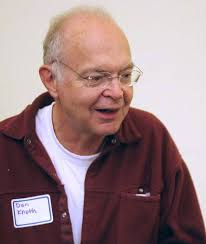
\includegraphics[width=.4\textwidth]{img/knuth.jpg}
	\caption{Donald Knuth}
	\label{fig:knuth}
\end{figure}


\begin{figure}[!htb]
	\centering
	\includegraphics[width=.4\textwidth]{img/783px-Test-Logo.svg}
	\caption{Test}
	\label{fig:test}
\end{figure}

Abbildungen bindet man mit \verb=\includegraphics= in einer Umgebung
\verb=figure= ein.
Man kann dann im Text auf die Abbildung \ref{fig:knuth} verweisen.
Man muss beachten, dass die Abbildung in einer sogenannten
\enquote{fließenden} Umgebung eingebunden wird, d.h. beim Setzen des
Dokuments bestimmt \TeX, an welcher Stelle genau im Dokument die
Abbildung erscheint.

Wie man an diesem Beispiel sieht, kann man beliebige Abbildungen etwa
\verb=jpg= wie in diesem Beispiel, aber auch \verb=pdf= einbinden. Man
kann also Abbildungen mit einem Grafikprogramm erstellen, als
\verb=pdf= speichern und dann einbinden.

\newcommand{\tikz}{Ti\emph{k}Z}

Es gibt aber auch \tikz\ (= \tikz\ ist kein Zeichenprogramm), das der
deutsche Informatiker Till Tantau entwickelt hat. Damit ist es möglich,
Abbildungen zu \enquote{programmieren}. Die Projektseite von \tikz\ ist
\url{https://sourceforge.net/projects/pgf/}. Interessant sind auch
die Beispiele auf \url{http://www.texample.net/tikz/examples/}.

\section{Tabellen}

Tabellen werden in einer \enquote{fließenden} Umgebung namens
\verb=table= eingegeben. Der eigentliche Inhalt der Tabelle kommt in die
Umgebung \verb=tabular=.

\begin{table}[!htb]
	\centering
	\caption{Die Geschichte von \TeX\ und \LaTeX}
	\begin{tabular}{ r p{13cm}}
		\toprule
		Jahr & Entwicklung\\
		\midrule
		1977 & Donald Knuth beginnt mit der Entwicklung von \TeX.\\
		1985 & \LaTeX\ (mächtige Makros, die die Verwendung von \TeX\
			vereinfachen, in dem sie Struktur und Layout trennen) wird von
			Leslie Lamport in der Version 2.09 freigegeben.\\
		1986 & Feier der Fertigstellung von \TeX\ im Computer Museum in
		Boston\\
		1986 & Leslie Lamport veröffentlicht \emph{\LaTeX: A Document
			Preparation System}.\\
		1993 & \LaTeXe\\
		2000 & pdf\TeX\ (entwickelt von Hàn Thé Thành)\\
			?  & Nach dem Tod von Donald Knuth bekommt \TeX\ die Versionsnummer
			$\pi$.\\
		\bottomrule
	\end{tabular}
	\label{tbl:geschichte}
\end{table}

Wie man am Beispiel des \LaTeX-Texts der Tabelle  \ref{tbl:geschichte}
sieht, kann die Formatierung von Tabellen etwas \enquote{sperrig} sein.
Gut, dass man sich in einer der vielen Anleitungen dazu erkundigen kann,
z.B. in der \LaTeXe-Kurzbeschreibung \cite[S.23]{lkurz15}.

\section{Listings}

\verb=listings= ist ein Paket, das es erlaubt, Code-Beispiele in die
Abschlussarbeit zu setzen. Wie das Beispiel \ref{lst:datei} zeigt, kann
man auch externe Dateien einbinden und im Text verbatim einsetzen. In
diesem Fall kann der eingebundene Text auch in der Zeichenkodierung
\emph{utf8} sein, wohingegen dies bei direkt im Text geschriebenen
Codebeispielen nicht unterstützt wird.

\begin{lstlisting}[caption={Einbinden einer Quelldatei}\label{lst:datei}]
% Der Inhalt der Datei myclass.java wird verbatim hier eingefügt
\lstinputlisting[caption={Eine Java-Klasse}\label{lst:java}]{myclass.java}
\end{lstlisting}

Für Listings gibt es viele Optionen des Layouts, insbesondere ist es
möglich die Programmiersprache des eingebundenen Code-Beispiels
anzugeben, was dazu führt, dass Schlüsselworte, Bezeichner und Kommentare
der Sprache im Layout hervorgehoben werden.

\section{Mathematische Formeln}

Mathematisches kann man in den laufenden Text einbauen, wie etwa bei
folgender Definition:

Mit $k!$, der Fakultät einer natürlichen Zahl $k$ bezeichnet man das
Produkt $1 \cdot 2 \cdot \dotso \cdot k$.

Oft braucht man aber auch ganze Abschnitte im Mathematik-Modus, wie in
folgendem Beispiel:

		Die sogenannte Collatz-Folge\footnote{ nach Lothar Collatz,
		deutscher Mathematiker 1910 - 1990} zu einer natürlichen Zahl $n$
		wird folgendermaßen gebildet:

	\begin{align}
	  n_1 &= n \nonumber \\
		n_{i+1} &= \left\{ \begin{array}{l l}
	                   n_i/2      & \textrm{falls $n_i$ gerade}\\
										 3 n_i + 1  & \textrm{falls $n_i$ ungerade}
										 \end{array} \right. \nonumber
	\end{align}

	\medskip
										 
	Startet man etwa mit der Zahl $7$ erhält man

	\[7\ 22\ 11\ 34\ 17\ 52\ 26\ 13\ 40\ 20\ 10\ 5\ 16\ 8\ 4\ 2\ 1\ 4\ 2\ 1\ \dots\]

	Wie man sieht, geht die Folge schließlich in den Zyklus $1, 4, 2$
	über.  Die \emph{Collatz-Vermutung} besagt, dass dies für jeden
	Startwert $n$ der Fall ist, d.h.  jede Collatz-Folge erreicht
	irgendwann den Wert $1$.

Mehr über das Setzen von mathematischen Formeln steht in \cite[Kapitel 4]{lkurz15}.



% ----------------------------------------------------------------------------
    % Kapitel 3

\end{lstlisting}

% ----------------------------------------------------------------------------

%% ----------------------------------------------------------------------------
% Copyright (c) 2016 -2020 by Burkhardt Renz. All rights reserved.
% Die Vorlage für eine Abschlussarbeit in der Informatik am Fachbereich
% MNI der THM ist lizenziert unter einer Creative Commons
% Namensnennung-Nicht kommerziell 4.0 International Lizenz.
%
% Id:$
% ----------------------------------------------------------------------------

\chapter{Elemente für die Gliederung}

Der Text dieses Kapitels steht in \verb=gliederung.tex=. Er bezieht sich
auf \verb=vorlage.tex= und \verb=gliederung.tex=.

\section{Teile}

Eine Abschlussarbeit besteht aus drei großen Teilen:

\begin{itemize}
	\item Dem Vorderteil (\verb=frontmatter=) mit
		\begin{itemize}
			\item der Titelseite,
			\item der eidesstattlichen Erklärung,
			\item der Zusammenfassung,
			\item dem Inhaltsverzeichnis und
			\item den Verzeichnissen von Abbildungen, Tabellen und Listings,
		\end{itemize}
	\item dem Hauptteil (\verb=mainmatter=) mit den Kapiteln der Arbeit
		und
	\item dem Anhang (\verb=backmatter=) mit Anhängen und dem
		Literaturverzeichnis	
\end{itemize}

Manchmal erwarten Dozentinnen oder Dozenten, dass eine Abschlussarbeit
Verzeichnisse der Abbildungen, Tabellen und Listings oder auch ein Glossar
der verwendeten Begriffe enthält. Deshalb enthält unsere Vorlage diese
Verzeichnisse. Ein Glossar kann man mit der Umgebung \verb=description=
oder \verb=labeling= erzeugen, die in Abschnitt
\ref{sec:stichwortlisten}  beschrieben werden.

Ich persönlich finde, dass man auf diese Verzeichnisse verzichten kann.
Und ein Glossar ist meines Erachtens nur nötig, wenn man viele
Fachbegriffe in der Arbeit verwendet, die einem in der Informatik
Kundigen nicht geläufig sind.

\section{Kapitel und ihre Untergliederungen}

Die Dokumentklasse \verb=scrbook= hat als Möglichkeiten der Gliederung
zunächst den Teil (\verb=part=). Er wird in diesem Dokument nicht
verwendet und meistens ist eine Bachelor- oder Masterarbeit nicht so
umfangreich, als dass man sie in Teile unterteilen müsste.

Die nächste Ebene ist das Kapital (\verb=chapter=), wie wir auf der
vorigen Seite den Anfang eines solchen sehen. Kapitel beginnen immer auf
einer rechten Seite.

Dann kommt der Abschnitt (\verb=section=) --- in einem solchen befinden wir
uns im Moment.

\subsection{Unterabschnitt}

Dies ist eine \verb=subsection=.

\subsubsection{Unterunterabschnitt}

Jetzt sind wir noch eine Ebene tiefer, in der \verb=subsubsection=. Eine
Gliederung sollte ausgewogen sein, auch in Bezug auf die
Gliederungstiefe. Deshalb sollte man eher nicht bis zum
Unterunterabschnitt gehen.


\paragraph{Absatz mit Überschrift}

Dies ist ein Absatz mit Überschrift \verb=paragraph=. Die Überschrift
wird im Dokument hervorgehoben, hat aber keine eigene Zeile. Typografen
nennen das auch einen \enquote{Spieß}.

\subparagraph{Unterabsatz}

Dies ist ein Unterabsatz \verb=subparagraph=, auch ein \enquote{Spieß}.

\section{Untergliederungen im Text}

\subsection{Aufzählungen}

Man kann nummerierte Aufzählungen mit der Umgebung \verb=enumerate=
erzeugen. Dies eignet sich für Aufzählungen, die eine Reihenfolge haben
und ist oft einer Aneinanderreihung im Text vorzuziehen, weil
übersichtlicher.

Eine Bachelorarbeit besteht aus

\begin{enumerate}
	\item einem ersten Kapitel
		\begin{enumerate}
			\item einem ersten Abschnitt darin,
			\item einem zweiten Abschnitt darin,
		\end{enumerate}
	\item einem zweiten Kapitel
	\item usw. usf.	
\end{enumerate}

Aufzählungen, die keine inhaltliche Reihenfolge haben, kann man mit der
Umgebung \verb=itemize= darstellen:

\begin{itemize}
	\item eine wichtige Aussage
	\item noch eine wichtige Aussage
		\begin{itemize}
			\item mit einer Ausprägung
			\item und noch einer Ausprägung	
		\end{itemize}
	\item \dots
\end{itemize}

\subsection{Stichwortlisten}
\label{sec:stichwortlisten}

Ein Beispiel für die Umgebung \verb=description= habe ich aus der
Dokumentation von \textsf{KOMA-Script} übernommen:

\begin{description}
	\item[empty] ist der Seitenstil, bei dem Kopf- und Fußzeile vollständig 
		leer bleiben. 
	\item[plain] ist der Seitenstil, bei dem keinerlei Kolumnentitel verwendet wird. 
	\item[headings] ist der Seitenstil für automatische Kolumnentitel. 
	\item[myheadings] ist der Seitenstil für manuelle Kolumnentitel. 
\end{description}

Es gibt auch noch die Umgebung \verb=labeling=, bei der man durch ein
Muster angeben kann, wie breit die Einrückung ist. Im Beispiel mit den
Seitenstilen könnte man das so machen:

\setkomafont{labelinglabel}{\sffamily\bfseries}
\begin{labeling}{myheadings}
	\item[empty] ist der Seitenstil, bei dem Kopf- und Fußzeile vollständig 
		leer bleiben. 
	\item[plain] ist der Seitenstil, bei dem keinerlei Kolumnentitel verwendet wird. 
	\item[headings] ist der Seitenstil für automatische Kolumnentitel. 
	\item[myheadings] ist der Seitenstil für manuelle Kolumnentitel. 
\end{labeling}

\section{Zum Literaturverzeichnis}

In der Vorlage findet man das Literaturverzeichnis in der Datei
\verb=litverz.tex=. 

Das Literaturverzeichnis kann man in \LaTeX\ auf zwei Arten erstellen:

Die einfache Variante besteht darin, dass man die Umgebung
\verb=bibliography= verwendet. So haben wir das in diesem Dokument
gemacht. Die Angaben zur Literatur stehen in \verb=litverz=. Jeder
Eintrag hat einen \emph{key}, den wir im Text im Befehl \verb=\cite=
referenzieren können. Die Referenz wird dann als Nummer im Text
angegeben und die entsprechende Nummer erscheint auch im
Literaturverzeichnis.

Die etwas aufwändigere Variante besteht darin, \verb=bibtex= zu
verwenden. Dies lohnt sich insbesondere dann, wenn man in verschiedenen
Manuskripte immer wieder dieselben Literaturverweise verwendet.

Mit \verb=bibtex= speichert man die Literaturangaben in einer Art
Datenbank, einer BibTeX-Datei. Die im Manuskript referenzierten Arbeiten
werden dann von \verb=bibtex= automatisch in das Literaturverzeichnis
übernommen. Die Formatierung des Verweises im Text und der Einträge im
Literaturverzeichnis wird dabei durch eine eigene Datei, dem
BibTeX-Stil, gesteuert. Will man die Verweise durch Nummern, wählt man
als Stil \verb=plain=, will man die Verweise durch die Abkürzung des
Autorennamens mit Angabe des Jahres, wählt man z.B. den Stil
\verb=alpha=. Es gibt eine Vielzahl solcher BibTeX-Stile, siehe
\url{https://www.ctan.org/tex-archive/biblio/bibtex/contrib}. Man kann sogar
eigene BibTeX-Stile definieren mit \verb=tex makebst=.

Mehr über BibTeX findet man z.B. bei \url{https://de.wikibooks.org/wiki/LaTeX-Kompendium:_Zitieren_mit_BibTeX}.

% ----------------------------------------------------------------------------

%% ----------------------------------------------------------------------------
% Copyright (c) 2016 - 2020 by Burkhardt Renz. All rights reserved.
% Die Vorlage für eine Abschlussarbeit in der Informatik am Fachbereich
% MNI der THM ist lizenziert unter einer Creative Commons
% Namensnennung-Nicht kommerziell 4.0 International Lizenz.
%
% Id:$
% ----------------------------------------------------------------------------

\chapter{Elemente im Text}

Der Text dieses Kapitels steht in \verb=elemente.tex= und bezieht auch
auf diese Datei.

\section{Typografische Elemente}

Im laufenden Text kann man alles Mögliche machen. Gute Typografie geht
mit diesen Möglichkeiten sparsam um. Was in Texten der Informatik oft
vorkommt ist die \emph{Hervorhebung} mit dem Befehl \verb=\emph=. Man
verwendet kursive Schrift auch für fremdsprachige Worte im Text, etwa
\textit{digital typography}.
Für Schlüsselworte, Befehle der Kommandozeile u.ä. nimmt man gerne einen
passenden Zeichensatz, etwa \texttt{make vorlage.pdf}. 

Das Paket \verb=csquotes= sorgt dafür dass Anführungszeichen
typografisch korrekt verwendet werden. Im Deutschen werden die
\enquote{Gänsefüßchen} nämlich anders als die angelsächsischen
\foreignquote{english}{quotation marks} gesetzt.

Mehr über das Setzen von Text findet man in \cite{lkurz15}.

\section{Referenzen und Links}

Verweise auf die Literatur macht man mit dem Befehl \verb=\cite=.
Braucht man Querverweise auf Abschnitte im Text oder Abbildungen etc.,
so versieht man das Verweisziel mit einem \verb=\label= und verweist
dann mit \verb=\ref= oder \verb=\pageref=. Mehr dazu in
\cite[S.50]{partosch15}.

Links auf Quellen im Internet werden durch den Befehl \verb=\url=
angegeben und dadurch in PDF \enquote{anklickbar}, etwa wie
\url{https://tug.org/mactex/src/WelcomeToMacTeX.pdf}.

\section{Abbildungen}

\begin{figure}[!htb]
	\centering
	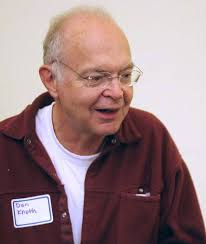
\includegraphics[width=.4\textwidth]{img/knuth.jpg}
	\caption{Donald Knuth}
	\label{fig:knuth}
\end{figure}


\begin{figure}[!htb]
	\centering
	\includegraphics[width=.4\textwidth]{img/783px-Test-Logo.svg}
	\caption{Test}
	\label{fig:test}
\end{figure}

Abbildungen bindet man mit \verb=\includegraphics= in einer Umgebung
\verb=figure= ein.
Man kann dann im Text auf die Abbildung \ref{fig:knuth} verweisen.
Man muss beachten, dass die Abbildung in einer sogenannten
\enquote{fließenden} Umgebung eingebunden wird, d.h. beim Setzen des
Dokuments bestimmt \TeX, an welcher Stelle genau im Dokument die
Abbildung erscheint.

Wie man an diesem Beispiel sieht, kann man beliebige Abbildungen etwa
\verb=jpg= wie in diesem Beispiel, aber auch \verb=pdf= einbinden. Man
kann also Abbildungen mit einem Grafikprogramm erstellen, als
\verb=pdf= speichern und dann einbinden.

\newcommand{\tikz}{Ti\emph{k}Z}

Es gibt aber auch \tikz\ (= \tikz\ ist kein Zeichenprogramm), das der
deutsche Informatiker Till Tantau entwickelt hat. Damit ist es möglich,
Abbildungen zu \enquote{programmieren}. Die Projektseite von \tikz\ ist
\url{https://sourceforge.net/projects/pgf/}. Interessant sind auch
die Beispiele auf \url{http://www.texample.net/tikz/examples/}.

\section{Tabellen}

Tabellen werden in einer \enquote{fließenden} Umgebung namens
\verb=table= eingegeben. Der eigentliche Inhalt der Tabelle kommt in die
Umgebung \verb=tabular=.

\begin{table}[!htb]
	\centering
	\caption{Die Geschichte von \TeX\ und \LaTeX}
	\begin{tabular}{ r p{13cm}}
		\toprule
		Jahr & Entwicklung\\
		\midrule
		1977 & Donald Knuth beginnt mit der Entwicklung von \TeX.\\
		1985 & \LaTeX\ (mächtige Makros, die die Verwendung von \TeX\
			vereinfachen, in dem sie Struktur und Layout trennen) wird von
			Leslie Lamport in der Version 2.09 freigegeben.\\
		1986 & Feier der Fertigstellung von \TeX\ im Computer Museum in
		Boston\\
		1986 & Leslie Lamport veröffentlicht \emph{\LaTeX: A Document
			Preparation System}.\\
		1993 & \LaTeXe\\
		2000 & pdf\TeX\ (entwickelt von Hàn Thé Thành)\\
			?  & Nach dem Tod von Donald Knuth bekommt \TeX\ die Versionsnummer
			$\pi$.\\
		\bottomrule
	\end{tabular}
	\label{tbl:geschichte}
\end{table}

Wie man am Beispiel des \LaTeX-Texts der Tabelle  \ref{tbl:geschichte}
sieht, kann die Formatierung von Tabellen etwas \enquote{sperrig} sein.
Gut, dass man sich in einer der vielen Anleitungen dazu erkundigen kann,
z.B. in der \LaTeXe-Kurzbeschreibung \cite[S.23]{lkurz15}.

\section{Listings}

\verb=listings= ist ein Paket, das es erlaubt, Code-Beispiele in die
Abschlussarbeit zu setzen. Wie das Beispiel \ref{lst:datei} zeigt, kann
man auch externe Dateien einbinden und im Text verbatim einsetzen. In
diesem Fall kann der eingebundene Text auch in der Zeichenkodierung
\emph{utf8} sein, wohingegen dies bei direkt im Text geschriebenen
Codebeispielen nicht unterstützt wird.

\begin{lstlisting}[caption={Einbinden einer Quelldatei}\label{lst:datei}]
% Der Inhalt der Datei myclass.java wird verbatim hier eingefügt
\lstinputlisting[caption={Eine Java-Klasse}\label{lst:java}]{myclass.java}
\end{lstlisting}

Für Listings gibt es viele Optionen des Layouts, insbesondere ist es
möglich die Programmiersprache des eingebundenen Code-Beispiels
anzugeben, was dazu führt, dass Schlüsselworte, Bezeichner und Kommentare
der Sprache im Layout hervorgehoben werden.

\section{Mathematische Formeln}

Mathematisches kann man in den laufenden Text einbauen, wie etwa bei
folgender Definition:

Mit $k!$, der Fakultät einer natürlichen Zahl $k$ bezeichnet man das
Produkt $1 \cdot 2 \cdot \dotso \cdot k$.

Oft braucht man aber auch ganze Abschnitte im Mathematik-Modus, wie in
folgendem Beispiel:

		Die sogenannte Collatz-Folge\footnote{ nach Lothar Collatz,
		deutscher Mathematiker 1910 - 1990} zu einer natürlichen Zahl $n$
		wird folgendermaßen gebildet:

	\begin{align}
	  n_1 &= n \nonumber \\
		n_{i+1} &= \left\{ \begin{array}{l l}
	                   n_i/2      & \textrm{falls $n_i$ gerade}\\
										 3 n_i + 1  & \textrm{falls $n_i$ ungerade}
										 \end{array} \right. \nonumber
	\end{align}

	\medskip
										 
	Startet man etwa mit der Zahl $7$ erhält man

	\[7\ 22\ 11\ 34\ 17\ 52\ 26\ 13\ 40\ 20\ 10\ 5\ 16\ 8\ 4\ 2\ 1\ 4\ 2\ 1\ \dots\]

	Wie man sieht, geht die Folge schließlich in den Zyklus $1, 4, 2$
	über.  Die \emph{Collatz-Vermutung} besagt, dass dies für jeden
	Startwert $n$ der Fall ist, d.h.  jede Collatz-Folge erreicht
	irgendwann den Wert $1$.

Mehr über das Setzen von mathematischen Formeln steht in \cite[Kapitel 4]{lkurz15}.



% ----------------------------------------------------------------------------


\backmatter 

\appendix
%% ----------------------------------------------------------------------------
% Copyright (c) 2016 - 2020 by Burkhardt Renz. All rights reserved.
% Die Vorlage für eine Abschlussarbeit in der Informatik am Fachbereich
% MNI der THM ist lizenziert unter einer Creative Commons
% Namensnennung-Nicht kommerziell 4.0 International Lizenz.
%
% Id:$
% ----------------------------------------------------------------------------

\chapter{Installation von \LaTeX}

Der Text dieses Anhangs steht in \verb=install.tex=.

\section{Windows}

\subsection*{Installationsschritte}

\begin{enumerate}
	\item Downloadseite von MiKTeX \url{http://www.miktex.org/download}.

	\item Die Basisversion \textbf{Basic MiKTeX 2.9 Installer} herunterladen.

	\item Die Installationsdatei namens \verb=basic-miktex-2.9.xxxx.exe=  
		starten.
		
	\item Dem Installationswizard folgen (am einfachsten die
		vorgeschlagenen Werte für Verzeichnisse usw. übernehmen).

	\item	Einen Ordner für die eigenen Dokumente erstellen, z.B. in \emph{Eigene
Dokumente}.

\end{enumerate}

\subsection*{Erste Schritte mit \TeX works}

\begin{enumerate}
	\item Im Startmenü oder den Apps das Programm \emph{TeXworks} suchen
		und starten. Optional: Zur späteren Bequemlichkeit das Programm an die
		Taskleiste anheften. 

		Es erscheint das Editierfenster auf der linken Hälfte des Bildschirms.

	\item Zum ersten Ausprobieren im Menü \emph{File} den Unterpunkt \emph{New 
	 	from Template} auswählen und in dem dann erscheinenden Dialog \emph{Basic 
		LaTeX documents} und \emph{article.tex}

	\item	Die Datei wird im Editorfenster geöffnet. Um daraus das PDF-Dokument
		zu erstellen drückt man auf den grünen Button links oben.

		Nun öffnet sich ein Dialog zum Abspeichern des Dokuments. Danach:

	\item	Die LaTeX-Datei wird übersetzt. Im linken Fenster unten sieht man die
		Meldungen über den Fortschritt dieses Vorgangs. (Beim ersten Mal
		dauert das relativ lange, weil diverse Pakete für LaTeX aus dem
		Internet heruntergeladen werden.)

	\item	Nach einiger Zeit erscheint das Ergebnis in einem neuen Fenster auf
		der rechten Seite des Bildschirms.

	\item	Jetzt kann es losgehen: links editieren, Erstellen des Dokuments
		mit dem grünen Button starten und rechts das Ergebnis überprüfen.
\end{enumerate}


\section{Mac OSX}

\subsection*{Installation von Mac\TeX}

\begin{enumerate}
	\item Das Package MacTeX.pkg erhältlich bei
		\url{http://www.tug.org/mactex/} herunterladen.
	\item Öffnet man das Paket mit Doppelklick, startet die Installation
		und sie wird schrittweise durchgeführt.	
\end{enumerate}

\subsection*{Arbeiten mit TeXShop}

Nach der Installation hat man im Launchpad eine App namens TeXShop. Dies
ist ein Editor für \TeX\ und \LaTeX.

\section{Linux}

Die einfachste Variante besteht darin, eine komplette \TeX
Live-Installation durchzuführen mittels

\begin{lstlisting}
sudo apt-get install texlive-full
\end{lstlisting}

Dabei wird allerdings vieles installiert, das man voraussichtlich
niemals braucht. Andererseits muss man aber nicht wissen, was man
mindestens installieren muss, damit \LaTeX\ verwendet werden kann.

Auf Github findet man Skripte, die Installationen z.B. unter Ubuntu
steuern können. Beispiel:
\url{https://github.com/scottkosty/install-tl-ubuntu}. Ich habe aber
keine Ahnung, wie gut diese Skripte tatsächlich sind.

% ----------------------------------------------------------------------------

% ----------------------------------------------------------------------------
% Copyright (c) 2016 - 2020 by Burkhardt Renz. All rights reserved.
% Die Vorlage für eine Abschlussarbeit in der Informatik am Fachbereich
% MNI der THM ist lizenziert unter einer Creative Commons
% Namensnennung-Nicht kommerziell 4.0 International Lizenz.
%
% $Id: litverz.tex 979 2020-08-24 07:03:19Z br $
% ----------------------------------------------------------------------------

\begin{thebibliography}{99}

\bibitem{sigdestad22}
    Thomas Sigdestad
	\emph{Front-end frameworks: What is important right now?},
	\url{https://enonic.com/blog/front-end-frameworks-what-is-important},
    (abgerufen 26.04.2023)

\bibitem{googleTrends}
	---
	\emph{Google Trends JavaScript Frameworks},
	\url{https://trends.google.de/trends/explore/GEO_MAP/1682502600?hl=de&tz=-120&date=today+5-y&hl=de&q=%2Fm%2F012l1vxv,%2Fg%2F11c6w0ddw9,%2Fm%2F0j45p7w,%2Fg%2F11c0vmgx5d,%2Fm%2F0h94450&sni=3},
	(abgerufen 26.04.2023)

\bibitem{stackoverflowStats}
	---
	\emph{Stackoverflow Statistik zur Häufigkeit von Fragen nach Framework1},
	\url{https://insights.stackoverflow.com/trends?tags=reactjs%2Cangular%2Cvue.js%2Cember.js%2Cbackbone.js%2Cknockout.js%2Cangularjshttps://insights.stackoverflow.com/trends?tags=reactjs%2Cangular%2Cvue.js%2Cember.js%2Cbackbone.js%2Cknockout.js%2Cangularjs},
	(abgerufen 26.04.2023)

\bibitem{gackenheimer2015introduction}
	Cory Gackenheimer
	\emph{Introduction to React.},
	Apress,
	2015.

\bibitem{react}
	---
	\emph{React
	The library for web and native user interfaces},
	\url{https://react.dev/},
	(abgerufen 27.04.2023)

\bibitem{bin2019},
	Sufyan bin Uzayr, Nicholas Cloud , Tim Ambler
	\emph{JavaScript Frameworks for Modern Web Development}
	Springer,
	2019

\bibitem{vueFAQ}
	---
	\emph{Vue | Frequently Asked Questions},
	\url{https://vuejs.org/about/faq.html},
	(abgerufen 28.04.2023)
%not used
---
\bibitem{lkurz15}
	Marco Daniel, Patrick Gundlach, Walter Schmidt, Jörg Knappen, Hubert
	Partl und Irene Hyna
	\emph{\LaTeXe-Kurzbeschreibung},
	\url{http://mirror.unicorncloud.org/CTAN/info/lshort/german/l2kurz.pdf},
	2015.
\bibitem{knuth99}
	Donald E. Knuth
	\emph{The \TeX book},
  Reading, MA: Addison-Wesley,
	1986.
\bibitem{koma16}
	Markus Kohm
	\emph{Die Anleitung \textsf{KOMA-Script}},
	\url{http://www.komascript.de/~mkohm/scrguide.pdf}
	2016.
\bibitem{lamport94}
  Leslie Lamport
  \emph{\LaTeX: a document preparation system},
  2nd edition,
  Reading, MA: Addison-Wesley,
  1994.
\bibitem{partosch15}
	Günter Partosch
	\emph{Anforderungen an wissenschaftliche Abschlussarbeiten und wie sie
	mit \LaTeX\ gelöst werden können},
	\url{https://www.staff.uni-giessen.de/partosch/unterlagen/abschlussarbeit.pdf},
	2015.

\end{thebibliography}

% ----------------------------------------------------------------------------


\end{document}
% ----------------------------------------------------------------------------
